% Options for packages loaded elsewhere
\PassOptionsToPackage{unicode}{hyperref}
\PassOptionsToPackage{hyphens}{url}
\PassOptionsToPackage{dvipsnames,svgnames*,x11names*}{xcolor}
%
\documentclass[
  11pt,
]{krantz}
\usepackage{lmodern}
\usepackage{amssymb,amsmath}
\usepackage{ifxetex,ifluatex}
\ifnum 0\ifxetex 1\fi\ifluatex 1\fi=0 % if pdftex
  \usepackage[T1]{fontenc}
  \usepackage[utf8]{inputenc}
  \usepackage{textcomp} % provide euro and other symbols
\else % if luatex or xetex
  \usepackage{unicode-math}
  \defaultfontfeatures{Scale=MatchLowercase}
  \defaultfontfeatures[\rmfamily]{Ligatures=TeX,Scale=1}
\fi
% Use upquote if available, for straight quotes in verbatim environments
\IfFileExists{upquote.sty}{\usepackage{upquote}}{}
\IfFileExists{microtype.sty}{% use microtype if available
  \usepackage[]{microtype}
  \UseMicrotypeSet[protrusion]{basicmath} % disable protrusion for tt fonts
}{}
\makeatletter
\@ifundefined{KOMAClassName}{% if non-KOMA class
  \IfFileExists{parskip.sty}{%
    \usepackage{parskip}
  }{% else
    \setlength{\parindent}{0pt}
    \setlength{\parskip}{6pt plus 2pt minus 1pt}}
}{% if KOMA class
  \KOMAoptions{parskip=half}}
\makeatother
\usepackage{xcolor}
\IfFileExists{xurl.sty}{\usepackage{xurl}}{} % add URL line breaks if available
\IfFileExists{bookmark.sty}{\usepackage{bookmark}}{\usepackage{hyperref}}
\hypersetup{
  pdftitle={통계 패키지 활용},
  pdfauthor={한국한의학연구원, 구본초},
  colorlinks=true,
  linkcolor=Maroon,
  filecolor=Maroon,
  citecolor=Blue,
  urlcolor=Blue,
  pdfcreator={LaTeX via pandoc}}
\urlstyle{same} % disable monospaced font for URLs
\usepackage{color}
\usepackage{fancyvrb}
\newcommand{\VerbBar}{|}
\newcommand{\VERB}{\Verb[commandchars=\\\{\}]}
\DefineVerbatimEnvironment{Highlighting}{Verbatim}{commandchars=\\\{\}}
% Add ',fontsize=\small' for more characters per line
\usepackage{framed}
\definecolor{shadecolor}{RGB}{248,248,248}
\newenvironment{Shaded}{\begin{snugshade}}{\end{snugshade}}
\newcommand{\AlertTok}[1]{\textcolor[rgb]{0.33,0.33,0.33}{#1}}
\newcommand{\AnnotationTok}[1]{\textcolor[rgb]{0.37,0.37,0.37}{\textbf{\textit{#1}}}}
\newcommand{\AttributeTok}[1]{\textcolor[rgb]{0.61,0.61,0.61}{#1}}
\newcommand{\BaseNTok}[1]{\textcolor[rgb]{0.06,0.06,0.06}{#1}}
\newcommand{\BuiltInTok}[1]{#1}
\newcommand{\CharTok}[1]{\textcolor[rgb]{0.5,0.5,0.5}{#1}}
\newcommand{\CommentTok}[1]{\textcolor[rgb]{0.37,0.37,0.37}{\textit{#1}}}
\newcommand{\CommentVarTok}[1]{\textcolor[rgb]{0.37,0.37,0.37}{\textbf{\textit{#1}}}}
\newcommand{\ConstantTok}[1]{\textcolor[rgb]{0,0,0}{#1}}
\newcommand{\ControlFlowTok}[1]{\textcolor[rgb]{0.27,0.27,0.27}{\textbf{#1}}}
\newcommand{\DataTypeTok}[1]{\textcolor[rgb]{0.27,0.27,0.27}{#1}}
\newcommand{\DecValTok}[1]{\textcolor[rgb]{0.06,0.06,0.06}{#1}}
\newcommand{\DocumentationTok}[1]{\textcolor[rgb]{0.37,0.37,0.37}{\textbf{\textit{#1}}}}
\newcommand{\ErrorTok}[1]{\textcolor[rgb]{0.14,0.14,0.14}{\textbf{#1}}}
\newcommand{\ExtensionTok}[1]{#1}
\newcommand{\FloatTok}[1]{\textcolor[rgb]{0.06,0.06,0.06}{#1}}
\newcommand{\FunctionTok}[1]{\textcolor[rgb]{0,0,0}{#1}}
\newcommand{\ImportTok}[1]{#1}
\newcommand{\InformationTok}[1]{\textcolor[rgb]{0.37,0.37,0.37}{\textbf{\textit{#1}}}}
\newcommand{\KeywordTok}[1]{\textcolor[rgb]{0.27,0.27,0.27}{\textbf{#1}}}
\newcommand{\NormalTok}[1]{#1}
\newcommand{\OperatorTok}[1]{\textcolor[rgb]{0.43,0.43,0.43}{\textbf{#1}}}
\newcommand{\OtherTok}[1]{\textcolor[rgb]{0.37,0.37,0.37}{#1}}
\newcommand{\PreprocessorTok}[1]{\textcolor[rgb]{0.37,0.37,0.37}{\textit{#1}}}
\newcommand{\RegionMarkerTok}[1]{#1}
\newcommand{\SpecialCharTok}[1]{\textcolor[rgb]{0,0,0}{#1}}
\newcommand{\SpecialStringTok}[1]{\textcolor[rgb]{0.5,0.5,0.5}{#1}}
\newcommand{\StringTok}[1]{\textcolor[rgb]{0.5,0.5,0.5}{#1}}
\newcommand{\VariableTok}[1]{\textcolor[rgb]{0,0,0}{#1}}
\newcommand{\VerbatimStringTok}[1]{\textcolor[rgb]{0.5,0.5,0.5}{#1}}
\newcommand{\WarningTok}[1]{\textcolor[rgb]{0.37,0.37,0.37}{\textbf{\textit{#1}}}}
\usepackage{longtable,booktabs}
% Correct order of tables after \paragraph or \subparagraph
\usepackage{etoolbox}
\makeatletter
\patchcmd\longtable{\par}{\if@noskipsec\mbox{}\fi\par}{}{}
\makeatother
% Allow footnotes in longtable head/foot
\IfFileExists{footnotehyper.sty}{\usepackage{footnotehyper}}{\usepackage{footnote}}
\makesavenoteenv{longtable}
\usepackage{graphicx,grffile}
\makeatletter
\def\maxwidth{\ifdim\Gin@nat@width>\linewidth\linewidth\else\Gin@nat@width\fi}
\def\maxheight{\ifdim\Gin@nat@height>\textheight\textheight\else\Gin@nat@height\fi}
\makeatother
% Scale images if necessary, so that they will not overflow the page
% margins by default, and it is still possible to overwrite the defaults
% using explicit options in \includegraphics[width, height, ...]{}
\setkeys{Gin}{width=\maxwidth,height=\maxheight,keepaspectratio}
% Set default figure placement to htbp
\makeatletter
\def\fps@figure{htbp}
\makeatother
\usepackage[normalem]{ulem}
% Avoid problems with \sout in headers with hyperref
\pdfstringdefDisableCommands{\renewcommand{\sout}{}}
\setlength{\emergencystretch}{3em} % prevent overfull lines
\providecommand{\tightlist}{%
  \setlength{\itemsep}{0pt}\setlength{\parskip}{0pt}}
\setcounter{secnumdepth}{5}
\usepackage{kotex}
\usepackage{dhucs-cmap}
\usepackage{booktabs}
\usepackage{placeins}
\usepackage{enumerate}
\usepackage{amssymb}
\usepackage{amsmath}
\usepackage{mathtools}
\usepackage{float}
% \usepackage{setspace} \doublespacing
\usepackage{relsize}
\usepackage{bigints}
\usepackage{bm}
\usepackage{amsmath}
% \usepackage{titlesec}
\usepackage{lipsum}
\usepackage{longtable}
 \usepackage[font=small,labelfont=bf]{caption}
\usepackage{dcolumn}
\usepackage{array}
\usepackage{gensymb}
\usepackage{makecell}
\usepackage{multirow}
\usepackage{natbib}
\usepackage{rotating}
\usepackage[most]{tcolorbox}

\renewcommand\theadalign{cb}
\renewcommand\theadfont{\bfseries}
\renewcommand\theadgape{\Gape[4pt]}
\renewcommand\cellgape{\Gape[4pt]}
\DeclareMathAlphabet{\mathpzc}{OT1}{pzc}{m}{it}

\renewcommand\theadalign{cb}
\renewcommand\theadfont{\bfseries}
\renewcommand\theadgape{\Gape[4pt]}
\renewcommand\cellgape{\Gape[4pt]}

\newcolumntype{L}[1]{>{\raggedright\let\newline\\
\arraybackslash\hspace{0pt}}m{#1}}
\newcolumntype{C}[1]{>{\centering\let\newline\\
\arraybackslash\hspace{0pt}}m{#1}}
\newcolumntype{R}[1]{>{\raggedleft\let\newline\\
\arraybackslash\hspace{0pt}}m{#1}}
\newcolumntype{P}[1]{>{\raggedright\tabularxbackslash}p{#1}}
\newcommand{\specialcell}[2][c]{%
  \begin{tabular}[#1]{@{}c@{}}#2\end{tabular}}
\newcommand{\specialcelll}[2][l]{%
  \begin{tabular}[#1]{@{}l@{}}#2\end{tabular}}

\captionsetup[table]{aboveskip=0pt}
\captionsetup[table]{belowskip=10pt}

\linespread{1.5}

% \setmainfont[UprightFeatures={SmallCapsFont=AlegreyaSC-Regular}]{Alegreya}

\usepackage{framed,color}
\definecolor{shadecolor}{RGB}{248,248,248}

\renewcommand{\textfraction}{0.05}
\renewcommand{\topfraction}{0.8}
\renewcommand{\bottomfraction}{0.8}
\renewcommand{\floatpagefraction}{0.75}

% \renewenvironment{quote}{\begin{VF}}{\end{VF}}
\let\oldhref\href
\renewcommand{\href}[2]{#2\footnote{\url{#1}}}

\ifxetex
  \usepackage{letltxmacro}
  \setlength{\XeTeXLinkMargin}{1pt}
  \LetLtxMacro\SavedIncludeGraphics\includegraphics
  \def\includegraphics#1#{% #1 catches optional stuff (star/opt. arg.)
    \IncludeGraphicsAux{#1}%
  }%
  \newcommand*{\IncludeGraphicsAux}[2]{%
    \XeTeXLinkBox{%
      \SavedIncludeGraphics#1{#2}%
    }%
  }%
\fi

\makeatletter
\newenvironment{kframe}{%
\medskip{}
\setlength{\fboxsep}{.8em}
 \def\at@end@of@kframe{}%
 \ifinner\ifhmode%
  \def\at@end@of@kframe{\end{minipage}}%
  \begin{minipage}{\columnwidth}%
 \fi\fi%
 \def\FrameCommand##1{\hskip\@totalleftmargin \hskip-\fboxsep
 \colorbox{shadecolor}{##1}\hskip-\fboxsep
     % There is no \\@totalrightmargin, so:
     \hskip-\linewidth \hskip-\@totalleftmargin \hskip\columnwidth}%
 \MakeFramed {\advance\hsize-\width
   \@totalleftmargin\z@ \linewidth\hsize
   \@setminipage}}%
 {\par\unskip\endMakeFramed%
 \at@end@of@kframe}
\makeatother

\makeatletter
\@ifundefined{Shaded}{
}{\renewenvironment{Shaded}{\begin{kframe}}{\end{kframe}}}
\makeatother

\newenvironment{rmdblock}[1]
  {
  \begin{itemize}
  \renewcommand{\labelitemi}{
    \raisebox{-.7\height}[0pt][0pt]{
      {\setkeys{Gin}{width=3em,keepaspectratio}\includegraphics{images/#1}}
    }
  }
  \setlength{\fboxsep}{1em}
  \begin{kframe}
  \item
  }
  {
  \end{kframe}
  \end{itemize}
  }
  
\newenvironment{rmdnote}
  {\begin{rmdblock}{note}}
  {\end{rmdblock}}
  
\newenvironment{rmdcaution}
  {\begin{rmdblock}{caution}}
  {\end{rmdblock}}
  
\newenvironment{rmdimportant}
  {\begin{rmdblock}{important}}
  {\end{rmdblock}}
  
\newenvironment{rmdtip}
  {\begin{rmdblock}{tip}}
  {\end{rmdblock}}
  
\newenvironment{rmdwarning}
  {\begin{rmdblock}{warning}}
  {\end{rmdblock}}

\renewenvironment{quote}{\begin{kframe}}{\end{kframe}}

% \newenvironment{quoteshade}
%   {
%   \begin{itemize}
%   \begin{kframe}
%   \item
%   }
%   {
%   \end{kframe}
%   \end{itemize}
%   }
%   
% \newenvironment{rmdquote}
%  {\begin{quoteshade}}
%  {\end{quoteshade}}

\usepackage{makeidx}
\makeindex

\urlstyle{tt}

\usepackage{amsthm}
\makeatletter
\def\thm@space@setup{%
  \thm@preskip=8pt plus 2pt minus 4pt
  \thm@postskip=\thm@preskip
}
\makeatother

\frontmatter
\usepackage{booktabs}
\usepackage{longtable}
\usepackage{array}
\usepackage{multirow}
\usepackage{wrapfig}
\usepackage{float}
\usepackage{colortbl}
\usepackage{pdflscape}
\usepackage{tabu}
\usepackage{threeparttable}
\usepackage{threeparttablex}
\usepackage[normalem]{ulem}
\usepackage{makecell}
\usepackage{xcolor}
\usepackage[]{natbib}
\bibliographystyle{apalike}

\title{통계 패키지 활용}
\usepackage{etoolbox}
\makeatletter
\providecommand{\subtitle}[1]{% add subtitle to \maketitle
  \apptocmd{\@title}{\par {\large #1 \par}}{}{}
}
\makeatother
\subtitle{2020년도 2학기 충남대학교 정보통계학과 강의 노트}
\author{한국한의학연구원, 구본초}
\date{2020-09-19}

\begin{document}
\maketitle

{
\hypersetup{linkcolor=}
\setcounter{tocdepth}{2}
\tableofcontents
}
\listoftables
\listoffigures
\hypertarget{overview}{%
\chapter*{Course Overview}\label{overview}}


R을 이용한 데이터 분석 시 CRAN에 등록된 패키지를 활용한다. 적절한 패키지의 활용은 데이터 분석의 효율을 증대할 뿐 아니라 분석의 재현성을 향상할 수 있다. 본 강의는 지난학기에 학습한 통계프로그래밍언어 강의 내용의 연속선 상에서 진행할 예정이며, 해당 강의에서 학습한 내용들을 기반으로 데이터 분석 및 그 결과에 대한 보고서 작성, 그리고 R 생성 파일에 대한 버전 관리 방법에 대해 알아보고자 한다.

\hypertarget{purpose-course}{%
\subsubsection*{교과 목표}\label{purpose-course}}


\begin{quote}
\begin{itemize}
\tightlist
\item
  \textbf{R Markdown의 이해와 활용}
\item
  \textbf{R 프로그래밍 능력 향상 및 통계 시뮬레이션의 이해}
\item
  \textbf{R을 이용한 데이터 분석 실습}
\item
  \textbf{R을 이용한 기초 통계분석}
\item
  \textbf{텍스트 마이닝에 대한 이해}
\item
  \textbf{Shiny, plotly 를 활용한 동적 문서 및 시각화 이해}
\item
  \textbf{RStudio + Github을 이용한 버전관리 이해}
\end{itemize}
\end{quote}

\hypertarget{pre-course}{%
\subsubsection*{선수과목}\label{pre-course}}


\begin{quote}
\textbf{통계학 개론}
\textbf{통계 프로그래밍 언어}
\end{quote}

\hypertarget{course-method}
\item
  \textbf{실험/실습: 70 \%}
\end{itemize}

\hypertarget{grade-method}
\item
  \textbf{기말고사: 35 \%}
\item
  \textbf{출석: 10 \%}
\item
  \textbf{과제: 20 \%}
\end{itemize}
\end{quote}

\hypertarget{material-course}{%
\subsubsection*{교재}\label{material-course}}


\begin{quote}
별도의 교재 없이 본 강의 노트로 수업을 진행할 예정이며, 수업의 이해도 향상을 위해 아래 소개할 도서 및 웹 문서 등을 참고할 것을 권장함.
\end{quote}

\hypertarget{ref-course}{%
\subsubsection*{참고문헌}\label{ref-course}}


\begin{itemize}
\tightlist
\item
  \href{https://bookdown.org/yihui/rmarkdown-cookbook/}{R Markdown Cookbook} \citep{xie-2020}
\item
  \href{https://bookdown.org/yihui/bookdown/}{bookdown: Authoring Books and Technical Documents with R Markdown} \citep{xie-2016}
\item
  R과 knitr를 활용한 데이터 연동형 문서 만들기 \citep{ko-2014}
\item
  \href{https://r4ds.had.co.nz/}{R for data science} \citep{wickham-2016r}
\item
  Statistical Computing with R \citep{rizzo-2019}
\item
  \href{https://bookdown.org/rdpeng/rprogdatascience/}{R programming for data science} \citep{peng-2016}
\item
  \href{https://www.tidytextmining.com/}{Text mining with R} \citep{silge-2017}
\end{itemize}

\mainmatter

\hypertarget{r-markdown}{%
\chapter{R Markdown}\label{r-markdown}}

\begin{quote}
\textbf{Sketch}

\begin{itemize}
\tightlist
\item
  동일한 문서에 코드, 결과, 텍스트가 동시에 있을 수 있을까?
\item
  만약 결과와 도표가 자동으로 생성된 경우 데이터가 변경 되더라도 자동으로 문서를 업데이트 할 수 있을까?
\item
  최종 완료한 문서가 미래에도 열 수 있을까?
\item
  이러한 모든 과정이 매우 쉽다면??
\end{itemize}
\end{quote}

\footnotesize

\begin{figure}

{\centering 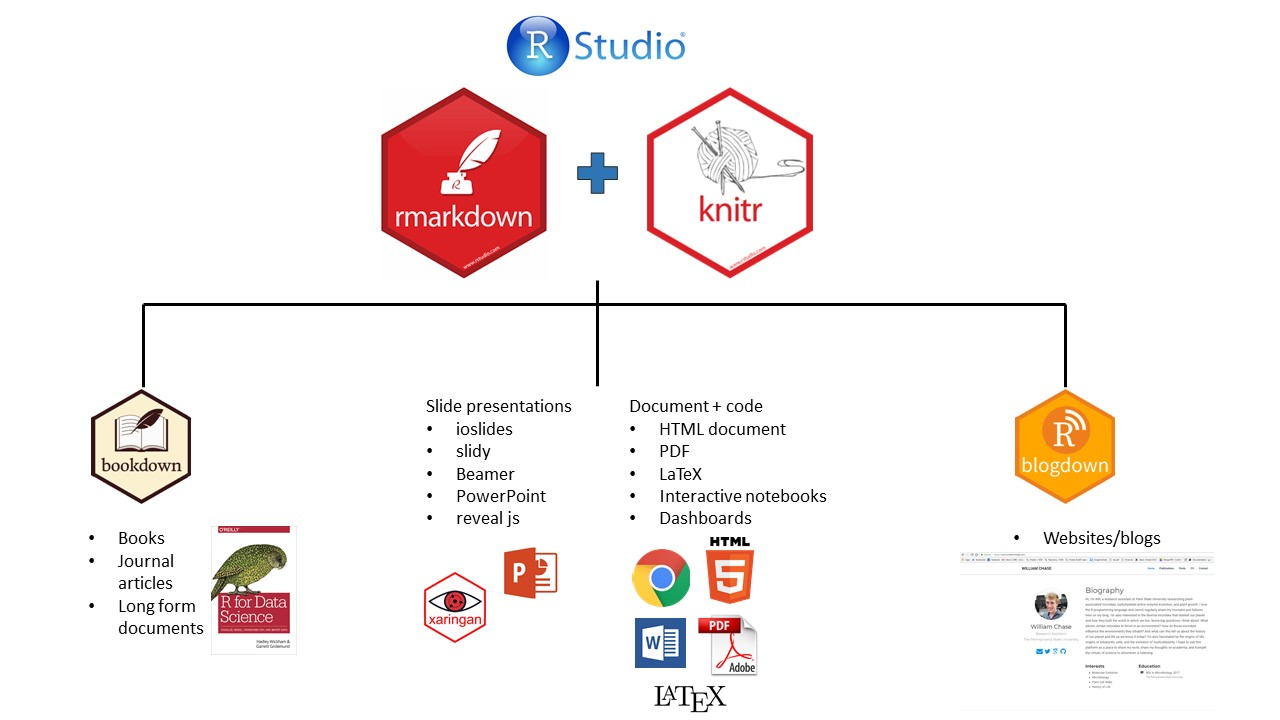
\includegraphics[width=1\linewidth]{figures/rmarkdown_universe} 

}

\caption{R markdown 세계(https://ulyngs.github.io/rmarkdown-workshop-2019 에서 발췌)}\label{fig:unnamed-chunk-1}
\end{figure}

\normalsize

\hypertarget{r-markdownuxc758-uxad6cuxc131}{%
\section{R Markdown의 구성}\label{r-markdownuxc758-uxad6cuxc131}}

\footnotesize

\begin{rmdnote}
본 절의 내용 중 일부는 지난 학기 강의노트 1.7절과 중복되거나 재구성한 내용이 포함됨.
\end{rmdnote}

\normalsize

\begin{enumerate}
\def\labelenumi{\arabic{enumi}.}
\tightlist
\item
  R Markdown은 R 코드와 분석 결과(표, 그림 등)을 포함한 문서 또는 컨텐츠를 제작하는 도구로 일반적으로 아래 열거한 형태로 활용함

  \begin{itemize}
  \tightlist
  \item
    문서 또는 논문(\texttt{pdf}, \texttt{html}, \texttt{docx})
  \item
    프리젠테이션(\texttt{pdf}, \texttt{html}, \texttt{pptx})
  \item
    웹 또는 블로그
  \end{itemize}
\item
  재현가능(reproducible)한 분석 및 연구\footnote{과학적 연구의 결과물을 오픈소스로 내놓고 누구라도 검증 가능} 가능

  \begin{itemize}
  \tightlist
  \item
    신뢰성 있는 문서 작성
  \item
    \texttt{Copy\ \&\ paste}를 하지 않고 효율적 작업 가능
  \end{itemize}
\end{enumerate}

\begin{quote}
\textbf{R 마크다운 파일 = \texttt{.Rmd} 확장자를 가진 일반 텍스트 파일}
\end{quote}

\begin{Shaded}
\begin{Highlighting}[]
\NormalTok{---}
\NormalTok{title: "Untitled.Rmd"}
\NormalTok{date: "2020-09-11"}
\NormalTok{output: html_document}
\NormalTok{---}

\BaseNTok{```\{r setup, include=FALSE\}}
\BaseNTok{knitr::opts_chunk$set(echo = TRUE)}
\BaseNTok{```}

\FunctionTok{## R Markdown}

\NormalTok{Markdown은 HTML, PDF 및 MS Word 문서를 작성하 기위한 간단한 형식 지정 구문입니다.}
\NormalTok{R Markdown 사용에 대한 자세한 내용은 }\OtherTok{<http://rmarkdown.rstudio.com>}\NormalTok{을 참조하십시오.}


\NormalTok{**Knit** 버튼을 클릭하면 두 가지를 모두 포함하는 문서가 생성됩니다.}
\NormalTok{문서에 포함 된 R 코드 청크의 출력 내용뿐 아니라}
\NormalTok{다음과 같이 R 코드 청크를 포함 할 수 있습니다.}

\BaseNTok{```\{r cars\}}
\BaseNTok{summary(cars)}
\BaseNTok{```}

\FunctionTok{## Including Plots}

\NormalTok{You can also embed plots, for example:}

\BaseNTok{```\{r pressure, echo=FALSE\}}
\BaseNTok{plot(pressure)}
\BaseNTok{```}

\BaseNTok{`echo = FALSE`}\NormalTok{ 매개 변수가 코드 청크에 추가되었습니다.}
\NormalTok{플롯을 생성 한 R 코드의 인쇄를 방지합니다.}
\end{Highlighting}
\end{Shaded}

위 R Markdown 문서는 아래 그림과 같이 \textbf{YAML}, \textbf{Markdown 텍스트}, \textbf{Code Chunk} 세 부분으로 구성됨.

\footnotesize

\begin{figure}

{\centering 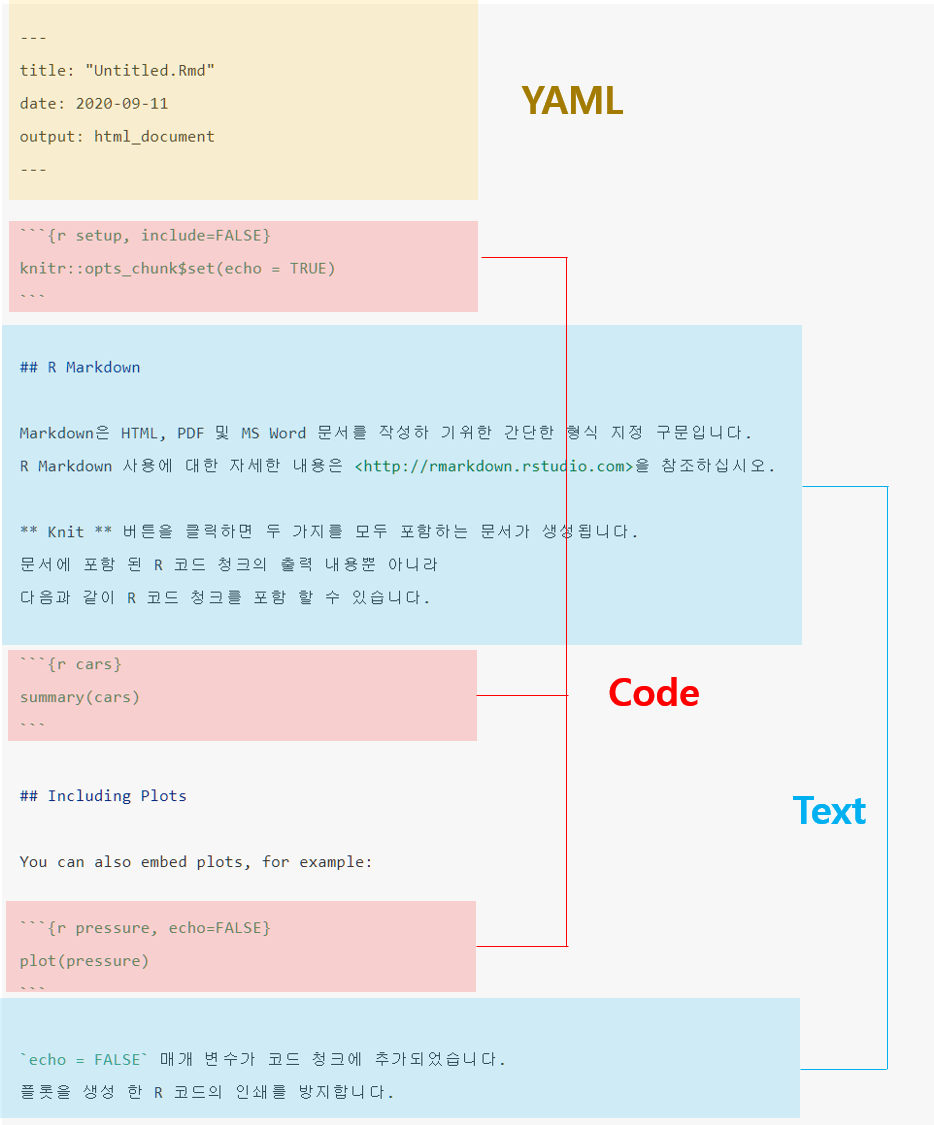
\includegraphics[width=1\linewidth]{figures/rmarkrdown-structure} 

}

\caption{R markdown structure}\label{fig:rmarkdown-structure}
\end{figure}

\normalsize

\textbf{YAML (YAML Ain't Markup Language)}

\begin{itemize}
\tightlist
\item
  R Markdown 문서의 metadata로 문서의 맨 처음에 항상 포함(header)되어야 함.
\item
  R Markdown 문서의 최종 출력 형태(\texttt{html}, \texttt{pdf}, \texttt{docx}, \texttt{pptx} 등), 제목, 저자, 날짜 등의 정보 등을 포함
\end{itemize}

\textbf{최종 문서 생성 과정}

\begin{itemize}
\tightlist
\item
  \texttt{Rmd} 파일을 \texttt{knitr} 을 통해 \texttt{.md} 파일로 변환 후 \texttt{pandoc} 이라는 문서 변환기를 통해 원하는 문서 포맷으로 출력
\end{itemize}

\footnotesize

\begin{figure}

{\centering 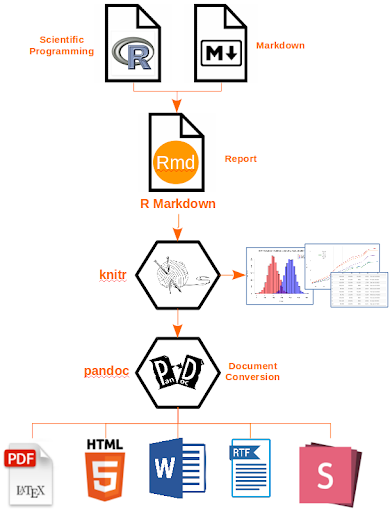
\includegraphics[width=0.6\linewidth]{figures/rmarkdown-flow} 

}

\caption{R Markdown의 최종 결과물 산출과정(http://applied-r.com/project-reporting-template/)}\label{fig:rmarkdown-flow}
\end{figure}

\normalsize

\hypertarget{r-markdown-uxbb38uxc11c-uxc2dcuxc791uxd558uxae30}{%
\section{R Markdown 문서 시작하기}\label{r-markdown-uxbb38uxc11c-uxc2dcuxc791uxd558uxae30}}

\begin{itemize}
\tightlist
\item
  \textbf{R Markdown} 문서 생성: \texttt{{[}File{]}\ -\textgreater{}\ {[}New\ File{]}\ -\textgreater{}\ {[}R\ Markdown..{]}}을 선택
\end{itemize}

\footnotesize

\begin{rmdcaution}
RStudio를 처음 설치하고 위와 같이 진행할 경우 아래와 같은 패키지 설치 여부를 묻는 팝업 창이 나타남. 패키지 설치 여부에 \texttt{{[}Yes{]}}를 클릭하면 R Markdown 문서 생성을 위해 필요한 패키지들이 자동으로 설치
\end{rmdcaution}

\normalsize

\footnotesize

\begin{center}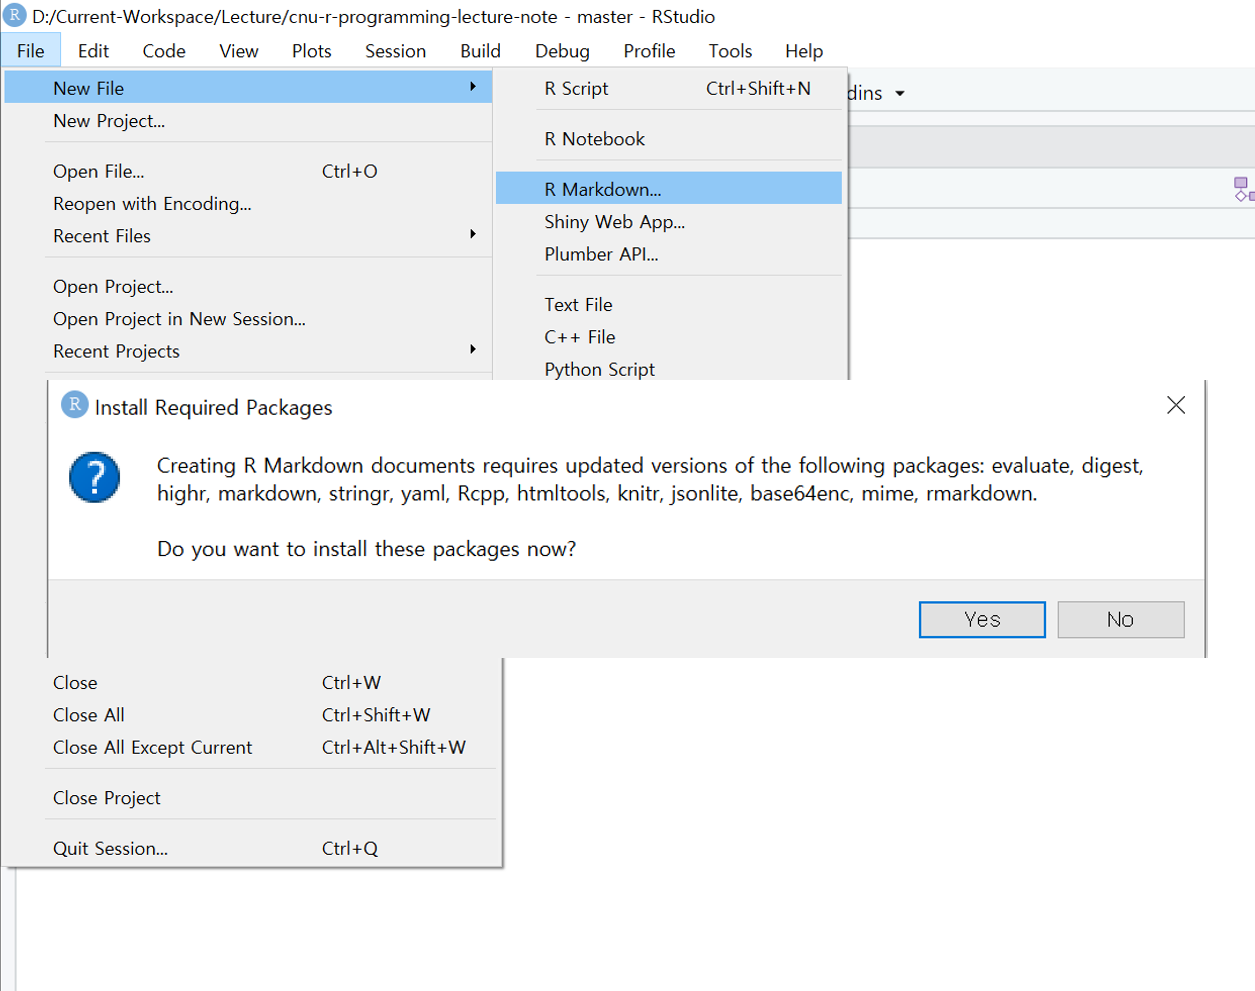
\includegraphics[width=0.8\linewidth]{figures/rmarkdown-new-01} \end{center}

\normalsize

\begin{itemize}
\tightlist
\item
  설치 완료 후 R Markdown으로 생성할 최종 문서 유형 선택 질의 창이 나타남. 아래 창에서 제목(Title)과 저자(Author) 이름 입력 후 \texttt{{[}OK{]}} 버튼 클릭(\texttt{Document}, \texttt{html} 문서 선택)
\end{itemize}

\footnotesize

\begin{center}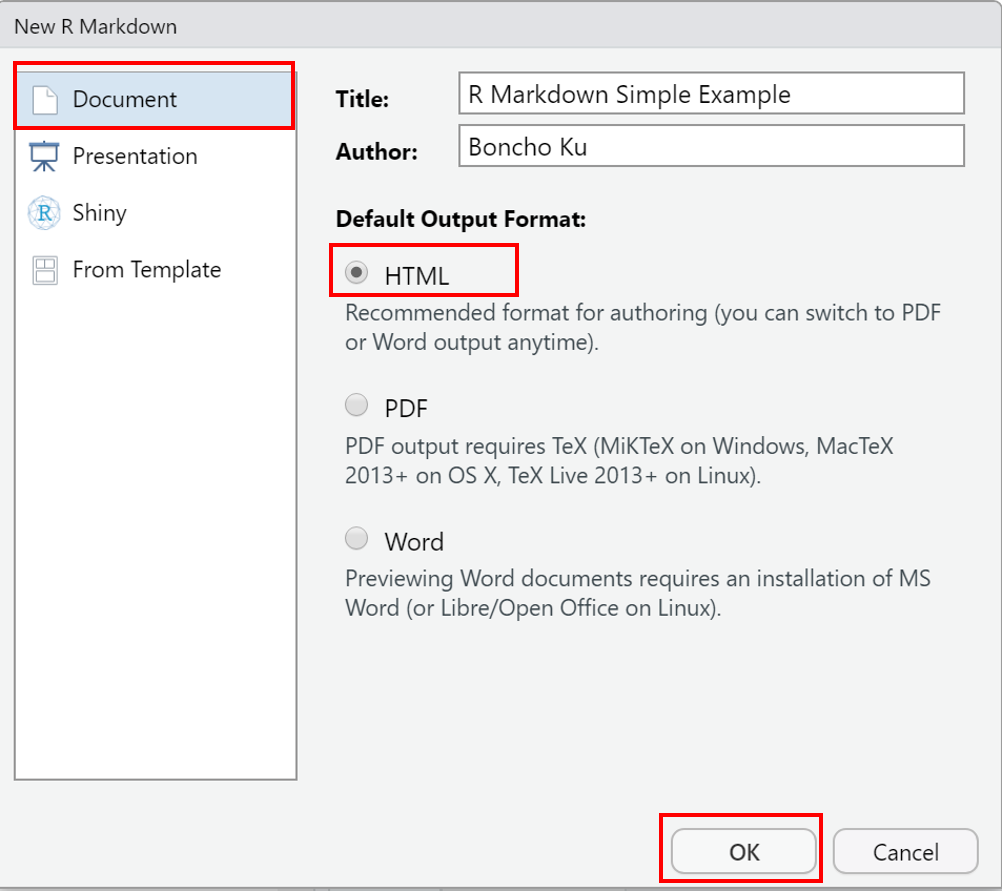
\includegraphics[width=0.8\linewidth]{figures/rmarkdown-new-02} \end{center}

\normalsize

\begin{itemize}
\tightlist
\item
  아래 그림과 같이 새로운 문서 창이 생성되고 \texttt{test.Rmd} 파일로 저장\footnote{{[}RStudio 프로젝트{]}에서 생성한 폴더 내에 파일 저장}
\end{itemize}

\footnotesize

\begin{center}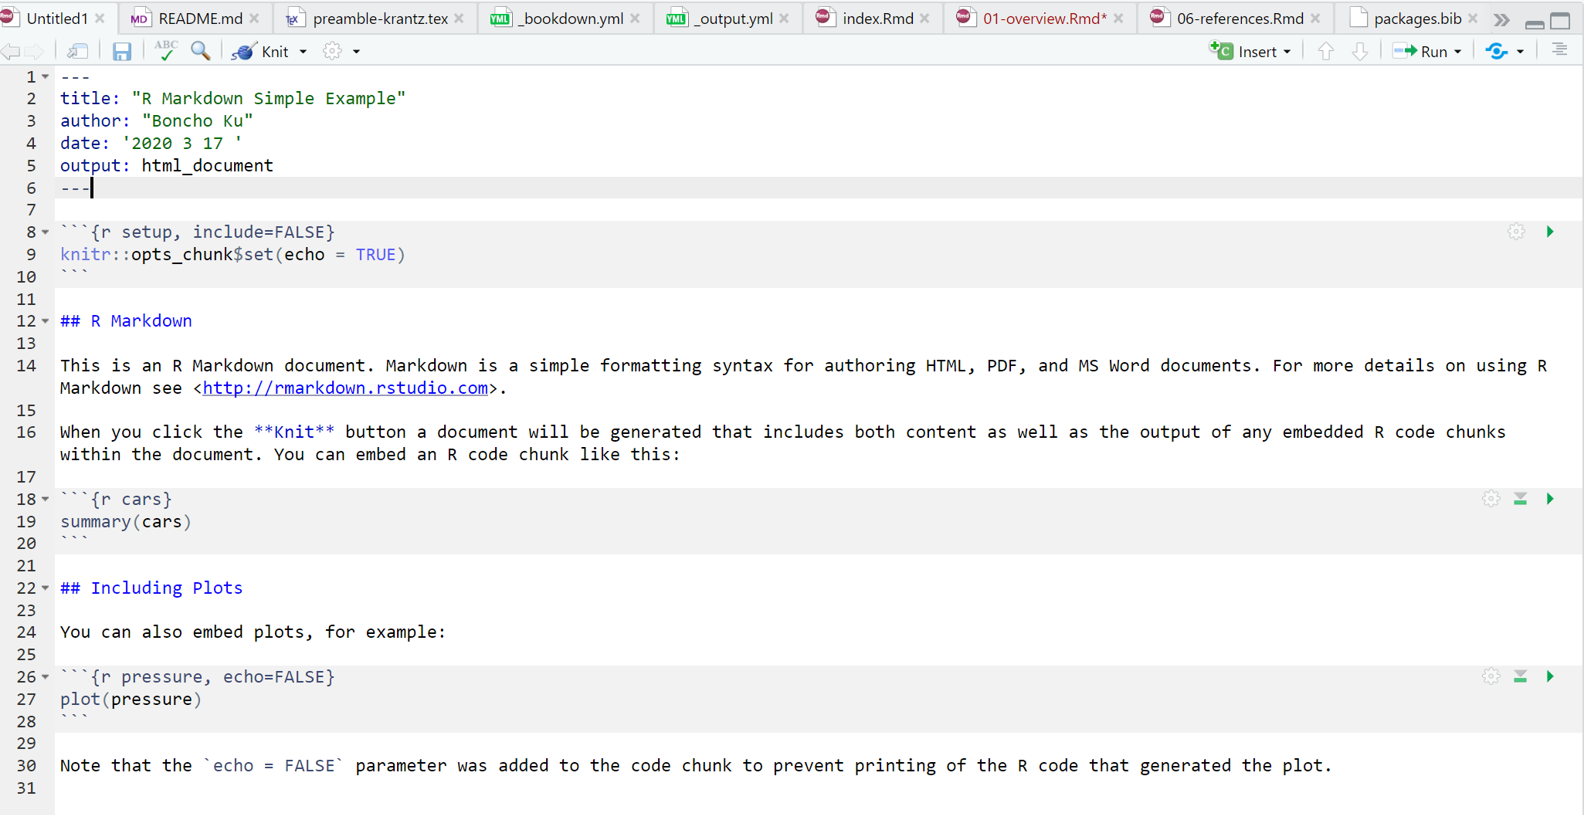
\includegraphics[width=0.8\linewidth]{figures/rmarkdown-new-03} \end{center}

\normalsize

\begin{itemize}
\tightlist
\item
  문서 상단에 \texttt{Knit} 아이콘을 클릭 후 \texttt{Knit\ to\ HTML} 클릭 또는 문서 아무 곳에 커서를 위치하고 단축키 \texttt{{[}Ctrl{]}\ +\ {[}Shift{]}\ +\ {[}K{]}} 입력
\end{itemize}

\footnotesize

\begin{center}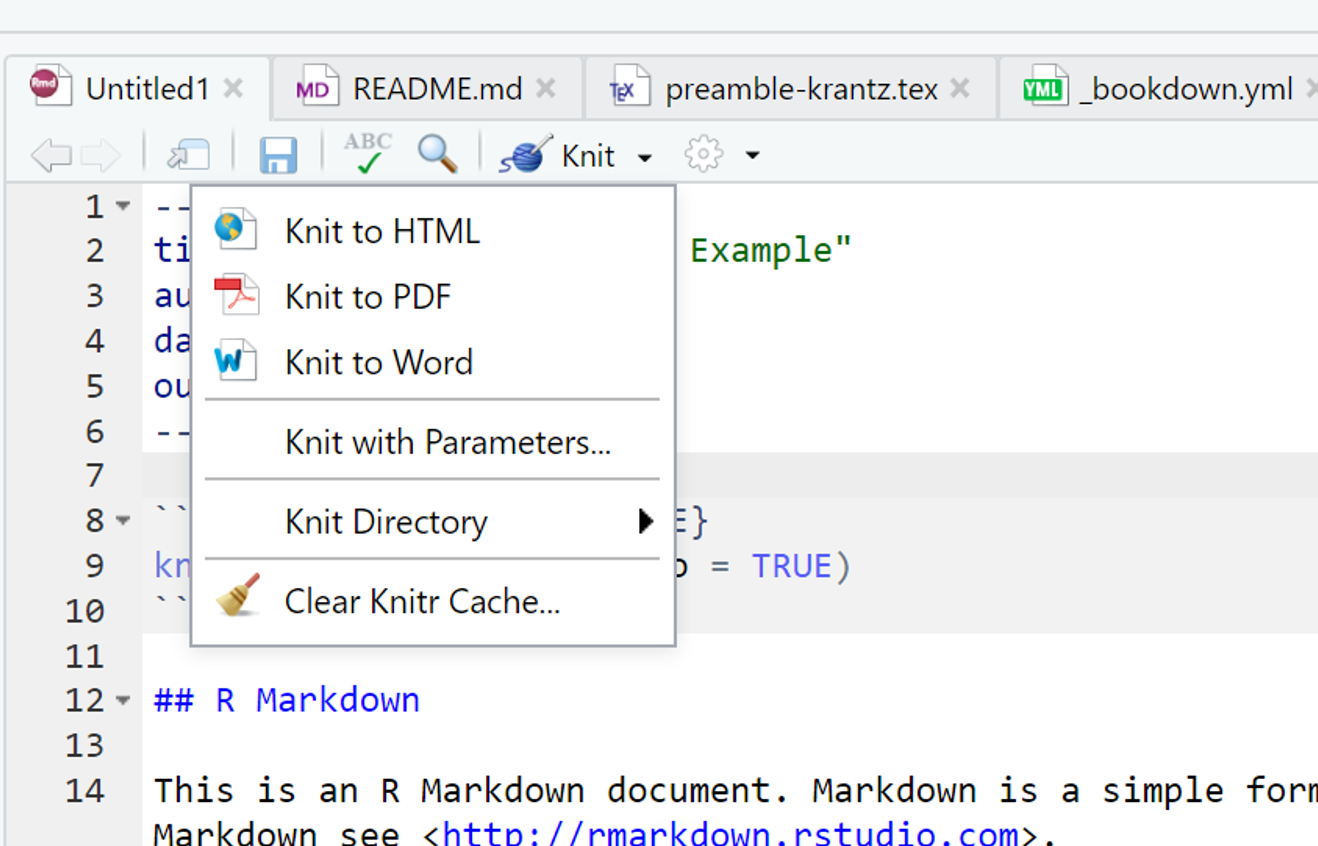
\includegraphics[width=0.8\linewidth]{figures/rmarkdown-new-04} \end{center}

\normalsize

\begin{itemize}
\tightlist
\item
  \texttt{knitr} + \texttt{R\ Markdown} + \texttt{pandoc} \(\rightarrow\) \texttt{html} 파일 생성 결과
\end{itemize}

\footnotesize

\begin{figure}

{\centering 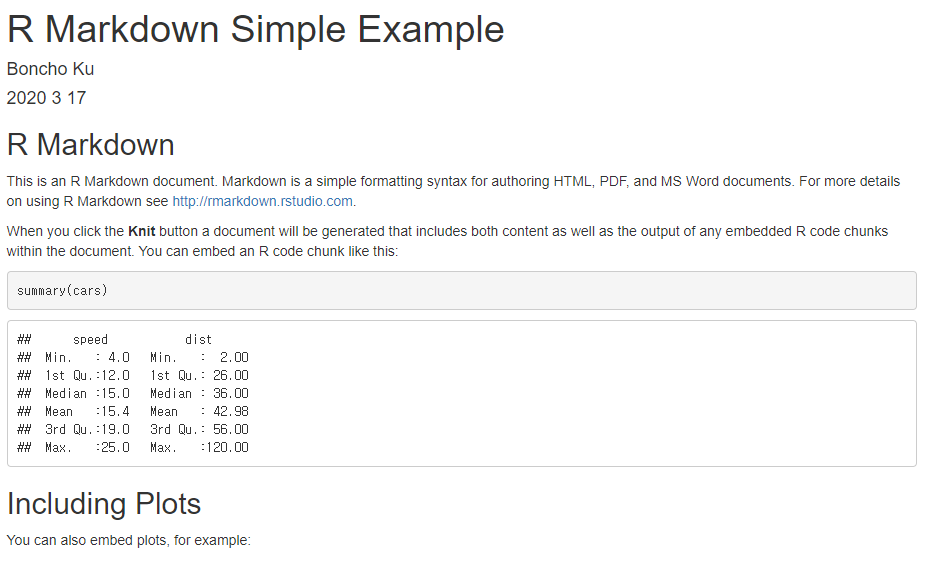
\includegraphics[width=0.8\linewidth]{figures/rmarkdown-new-out} 

}

\caption{test.html 문서 화면(저장 폴더 내 `test.html`을 크롬 브라우저로 실행)}\label{fig:rmarkdown-new-out}
\end{figure}

\normalsize

\hypertarget{r-markdown-uxae30uxbcf8-uxbb38uxbc95syntax}{%
\section{R Markdown 기본 문법(syntax)}\label{r-markdown-uxae30uxbcf8-uxbb38uxbc95syntax}}

\begin{quote}
R Markdown의 기본 문법은 Rstudio 풀다운 메뉴 \textbf{\texttt{{[}Help{]}}} \(\rightarrow\) \textbf{\texttt{{[}Markdown\ Quick\ Reference{]}}} 에서 확인 가능
\end{quote}

\hypertarget{uxd14duxc2a4uxd2b8-uxbb38uxbc95}{%
\subsection{텍스트 문법}\label{uxd14duxc2a4uxd2b8-uxbb38uxbc95}}

\textbf{강조(emphasis)}

\begin{itemize}
\tightlist
\item
  이텔릭체: *italic1*, \_italic2\_ \(\rightarrow\) \emph{italic1}, \emph{italic2}
\item
  볼드(굵은)체: *\emph{bold1*}, \_\_bold2\_\_ \(\rightarrow\) \textbf{bold1}, \textbf{bold2}
\end{itemize}

\textbf{Inline code}

\begin{itemize}
\tightlist
\item
  {`}inline code` \(\rightarrow\) \texttt{inline\ code}
\end{itemize}

\textbf{아래/위 첨자(sub/superscript)}

\begin{itemize}
\tightlist
\item
  subscript\textasciitilde2\textasciitilde{} \(\rightarrow\) subscript\textsubscript{2}
\item
  superscript\^{}2\^{} \(\rightarrow\) superscript\textsuperscript{2}
\end{itemize}

\textbf{삭제표시(strike through)}

\begin{itemize}
\tightlist
\item
  \textasciitilde\textasciitilde strikethrough\textasciitilde\textasciitilde{} \(\rightarrow\) \sout{strikethrough}
\end{itemize}

\textbf{생략표시(ellipsis)}

\begin{itemize}
\tightlist
\item
  ... \(\rightarrow\) \ldots{}
\end{itemize}

\textbf{긴/짧은 대쉬(en/emd-dash)}

\begin{itemize}
\tightlist
\item
  짧은 대쉬: -\/- \(\rightarrow\) --
\item
  긴 대쉬: -\/-\/- \(\rightarrow\) ---
\end{itemize}

\textbf{특수문자 탈출 지정자}

\begin{itemize}
\tightlist
\item
  \textbackslash*, \textbackslash\_, \textbackslash\textasciitilde, \textbackslash\textbackslash{} \(\rightarrow\) *, \_, \textasciitilde, \textbackslash{}
\end{itemize}

\textbf{하이퍼링크}

-\texttt{{[}text{]}(link)} \(\rightarrow\) \href{https://zorba78.github.io/cnu-r-programming-lecture-note}{통계프로그래밍언어}

\textbf{외부그림 삽입}

\begin{itemize}
\tightlist
\item
  \texttt{!{[}image\ title{]}(path/to/image)}: \texttt{!{[}장난꾸러기{]}(figures/son-02.jpg)}
\end{itemize}

\begin{figure}
\centering
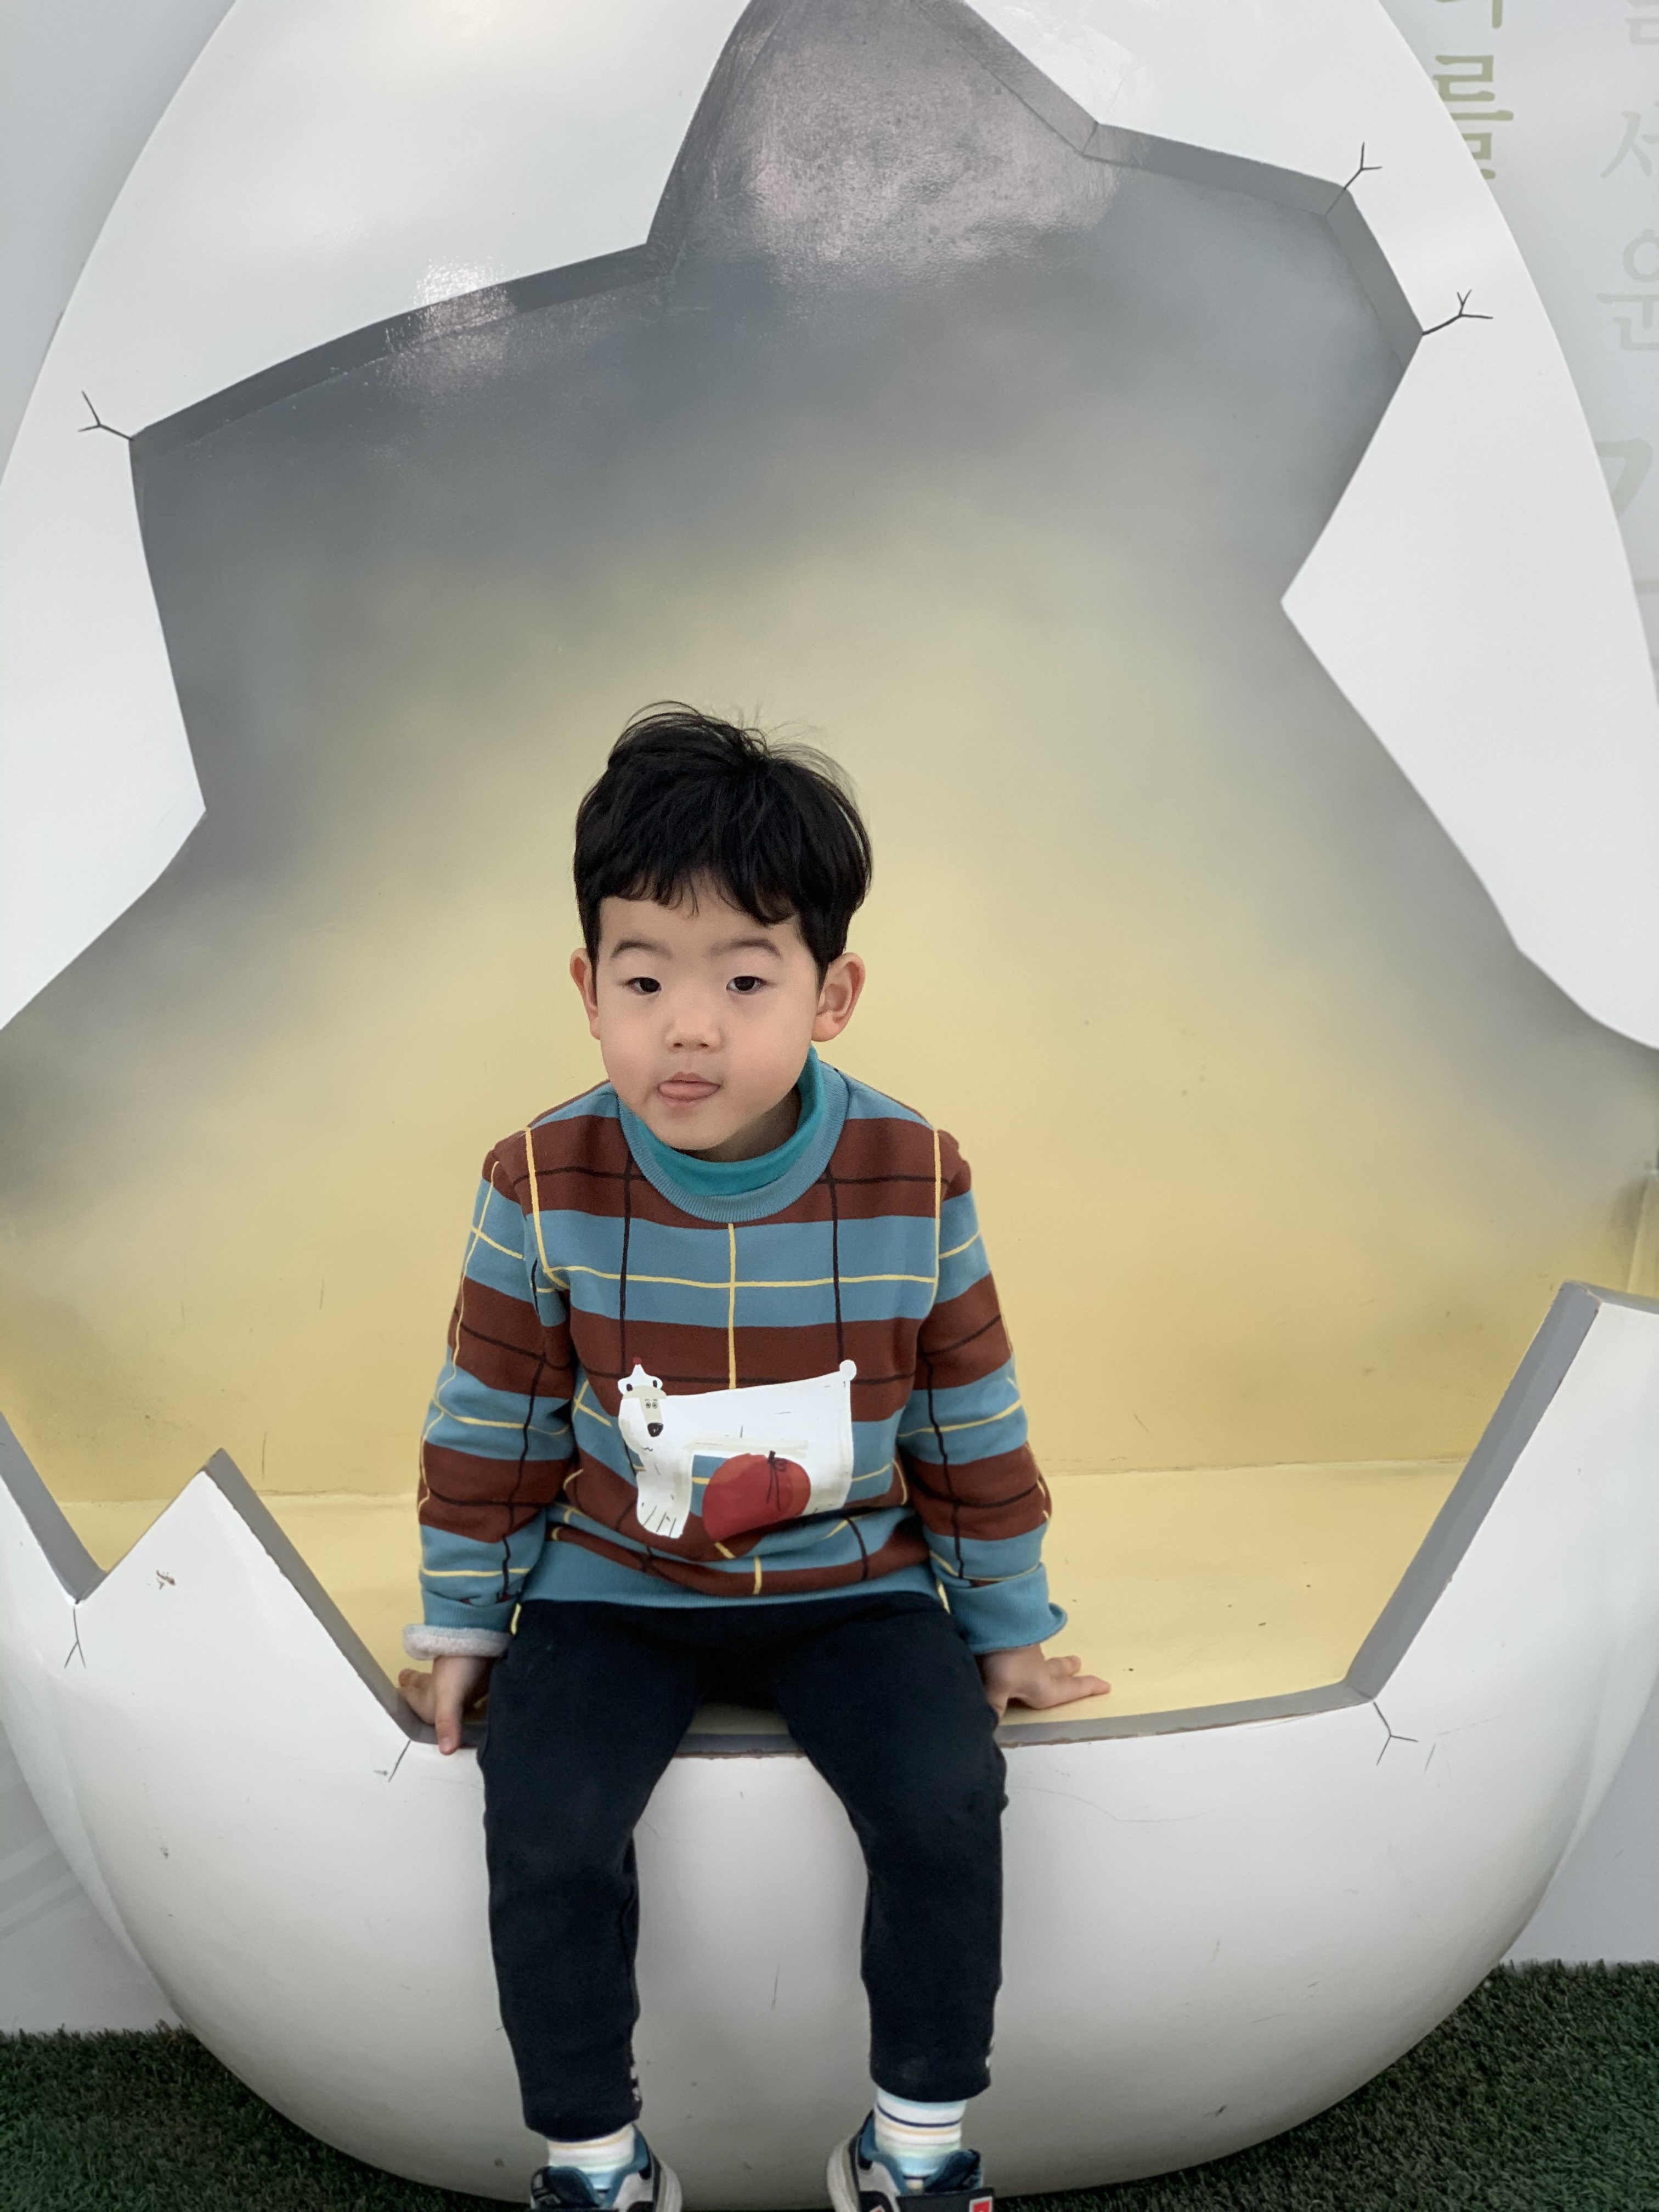
\includegraphics[width=0.8\textwidth,height=\textheight]{figures/son-02.jpg}
\caption{장난꾸러기}
\end{figure}

\textbf{강제 줄바꿈(line breaks)}

\begin{itemize}
\tightlist
\item
  하나의 줄에서 공백(space) 두 개 이상 또는 백슬레시(\texttt{\textbackslash{}}) 입력 후 \texttt{{[}Enter{]}}
\end{itemize}

\begin{Shaded}
\begin{Highlighting}[]
\NormalTok{End a line with two spaces to start }
\NormalTok{a new paragraph}
\end{Highlighting}
\end{Shaded}

End a line with two spaces to start
a new paragraph

\begin{Shaded}
\begin{Highlighting}[]
\NormalTok{End a line with two spaces to start\textbackslash{}}
\NormalTok{a new paragraph}
\end{Highlighting}
\end{Shaded}

End a line with two spaces to start\\
a new paragraph

\textbf{각주(footnote)}

\begin{itemize}
\tightlist
\item
  \texttt{A\ footnote\^{}{[}주석내용{]}} \(\rightarrow\) A footnote\footnote{주석내용}
\end{itemize}

\textbf{주석(comment)}

\begin{itemize}
\tightlist
\item
  \texttt{\textless{}!-\/-\ this\ is\ a\ comment\ that\ won\textquotesingle{}t\ be\ shown\ -\/-\textgreater{}} \(\rightarrow\) 
\end{itemize}

\footnotesize

\begin{rmdtip}
RStudio에서 단축키 \texttt{{[}Ctrl{]}} + \texttt{{[}Shift{]}} + \texttt{{[}C{]}}를 통해 전체 line 에 대해 주석처리 가능
\end{rmdtip}

\normalsize

\hypertarget{block-level-elements}{%
\subsection{Block-level elements}\label{block-level-elements}}

\textbf{장/절(header)}

\begin{itemize}
\tightlist
\item
  \# Header 1 (chapter, 장)
\item
  \#\# Header 2 (section, 절)
\item
  \#\#\# Header 3 (subsection, 관)
\end{itemize}

\textbf{목록(list)}

\begin{itemize}
\tightlist
\item
  비순서(unordered) 목록: \texttt{-}, \texttt{*}, \texttt{+} 중 어느 하나로 입력 가능
\end{itemize}

\begin{Shaded}
\begin{Highlighting}[]
\NormalTok{- }\StringTok{one item }
\StringTok{* two item}
\StringTok{   + sub-item 1}
\StringTok{   + sub-item 2}
\StringTok{      - subsub-item 1}
\StringTok{      - subsub-item 2}
\end{Highlighting}
\end{Shaded}

\begin{itemize}
\tightlist
\item
  one item
\item
  two item

  \begin{itemize}
  \tightlist
  \item
    sub-item 1
  \item
    sub-item 2

    \begin{itemize}
    \tightlist
    \item
      subsub-item 1
    \item
      subsub-item 2
    \end{itemize}
  \end{itemize}
\item
  순서(ordered) 목록: 비순서 목록의 기호 대신 숫자로 리스트 생성
\end{itemize}

\begin{Shaded}
\begin{Highlighting}[]
\NormalTok{1. }\StringTok{the first item}
\StringTok{   - sub-item 1}
\StringTok{2. the second item}
\StringTok{3. the third item}
\end{Highlighting}
\end{Shaded}

\begin{enumerate}
\def\labelenumi{\arabic{enumi}.}
\tightlist
\item
  the first item

  \begin{itemize}
  \tightlist
  \item
    sub-item 1
  \end{itemize}
\item
  the second item
\item
  the third item
\end{enumerate}

\begin{itemize}
\tightlist
\item
  같은 숫자로 적어도 순서대로 목록 생성
\end{itemize}

\begin{Shaded}
\begin{Highlighting}[]
\NormalTok{1. }\StringTok{the first item}
\StringTok{   - sub-item 1}
\StringTok{1. the second item}
\StringTok{1. the third item}
\end{Highlighting}
\end{Shaded}

\begin{enumerate}
\def\labelenumi{\arabic{enumi}.}
\tightlist
\item
  the first item

  \begin{itemize}
  \tightlist
  \item
    sub-item 1
  \end{itemize}
\item
  the second item
\item
  the third item
\end{enumerate}

\textbf{인용구(blockquote)}: \texttt{\textgreater{}}로 시작

\begin{Shaded}
\begin{Highlighting}[]
\NormalTok{>}\DataTypeTok{ "There are three kinds of lies: lies, damn lies, and statistics"}
\DataTypeTok{>}
\DataTypeTok{> --- Benjamin Disraeli}
\end{Highlighting}
\end{Shaded}

\begin{quote}
``There are three kinds of lies: lies, damn lies, and statistics''

\VA{--- Benjamin Disraeli}{}
\end{quote}

\hypertarget{uxc218uxc2dduxd45cuxd604math-expression}{%
\subsection{수식표현(math expression)}\label{uxc218uxc2dduxd45cuxd604math-expression}}

\begin{itemize}
\tightlist
\item
  줄 안에 수식 입력 시 \texttt{\$수식표현\$} 으로 입력
\item
  수식 display style (보통 교과서에 정리 및 정의에 기술된 수식들) 적용 시 \texttt{\$\$\ \textasciitilde{}\ \$\$} 안에 수식 입력
\item
  수식 표현은 LaTeX 의 수식 표현을 동일하게 준용(\url{https://www.latex4technics.com/}, \url{https://latex.codecogs.com/legacy/eqneditor/editor.php} 에서 수식 입력 명령어 학습 가능)
\item
  LaTeX 수식 입력 코드는
\item
  예시
\end{itemize}

\[
  P(X = x) = f(x; n, p) = {n \choose x} p^x (1-p)^{n-x}
\]

\begin{itemize}
\tightlist
\item
  Inline equation: \texttt{\$P(X\ =\ x)\ =\ f(x;\ n,\ p)\ =\ \{n\ \textbackslash{}choose\ x\}\ p\^{}x\ (1-p)\^{}\{n-x\}\$} \(\rightarrow\) \(P(X = x) = f(x; n, p) = {n \choose x} p^x (1-p)^{n-x}\)
\item
  Math block: \texttt{\$\$P(X\ =\ x)\ =\ f(x;\ n,\ p)\ =\ \{n\ \textbackslash{}choose\ x\}\ p\^{}x\ (1-p)\^{}\{n-x\}\$\$}
\end{itemize}

\[P(X = x) = f(x; n, p) = {n \choose x} p^x (1-p)^{n-x}\]

\begin{itemize}
\tightlist
\item
  \texttt{\$\ \$} 또는 \texttt{\$\$\ \$\$} 안에 LaTeX에서 제공하는 수식 함수 사용 가능
\end{itemize}

\begin{Shaded}
\begin{Highlighting}[]
\SpecialStringTok{$$}\SpecialCharTok{\textbackslash{}begin}\SpecialStringTok{\{array\}\{ccc\}}
\SpecialStringTok{x_\{11\} & x_\{12\} & x_\{13\}}\SpecialCharTok{\textbackslash{}\textbackslash{}}
\SpecialStringTok{x_\{21\} & x_\{22\} & x_\{23\}}
\SpecialCharTok{\textbackslash{}end}\SpecialStringTok{\{array\}$$}
\end{Highlighting}
\end{Shaded}

\[\begin{array}{ccc}
x_{11} & x_{12} & x_{13}\\
x_{21} & x_{22} & x_{23}
\end{array}\]

\begin{Shaded}
\begin{Highlighting}[]
\SpecialStringTok{$$}\SpecialCharTok{\textbackslash{}Theta}\SpecialStringTok{ = }\SpecialCharTok{\textbackslash{}begin}\SpecialStringTok{\{pmatrix\}}\SpecialCharTok{\textbackslash{}alpha}\SpecialStringTok{ & }\SpecialCharTok{\textbackslash{}beta\textbackslash{}\textbackslash{}}
\SpecialCharTok{\textbackslash{}gamma}\SpecialStringTok{ & }\SpecialCharTok{\textbackslash{}delta}
\SpecialCharTok{\textbackslash{}end}\SpecialStringTok{\{pmatrix\}$$}
\end{Highlighting}
\end{Shaded}

\[\Theta = \begin{pmatrix}\alpha & \beta\\
\gamma & \delta
\end{pmatrix}\]

\begin{Shaded}
\begin{Highlighting}[]
\SpecialStringTok{$$}\ErrorTok{\textbackslash{}begin\{align\}}\SpecialStringTok{ }
\SpecialStringTok{g(X_\{n\}) &= g(}\SpecialCharTok{\textbackslash{}theta}\SpecialStringTok{)+g'(\{}\SpecialCharTok{\textbackslash{}tilde}\SpecialStringTok{\{}\SpecialCharTok{\textbackslash{}theta}\SpecialStringTok{\}\})(X_\{n\}-}\SpecialCharTok{\textbackslash{}theta}\SpecialStringTok{) }\SpecialCharTok{\textbackslash{}notag}\SpecialStringTok{ }\SpecialCharTok{\textbackslash{}\textbackslash{}}
\SpecialCharTok{\textbackslash{}sqrt}\SpecialStringTok{\{n\}[g(X_\{n\})-g(}\SpecialCharTok{\textbackslash{}theta}\SpecialStringTok{)] &= g'}\SpecialCharTok{\textbackslash{}left}\SpecialStringTok{(\{}\SpecialCharTok{\textbackslash{}tilde}\SpecialStringTok{\{}\SpecialCharTok{\textbackslash{}theta}\SpecialStringTok{\}\}}\SpecialCharTok{\textbackslash{}right}\SpecialStringTok{)}
\SpecialStringTok{  }\SpecialCharTok{\textbackslash{}sqrt}\SpecialStringTok{\{n\}[X_\{n\}-}\SpecialCharTok{\textbackslash{}theta}\SpecialStringTok{ ]}
\ErrorTok{\textbackslash{}end\{align\}}\SpecialStringTok{$$}
\end{Highlighting}
\end{Shaded}

\[\begin{aligned} 
g(X_{n}) &= g(\theta)+g'({\tilde{\theta}})(X_{n}-\theta) \notag \\
\sqrt{n}[g(X_{n})-g(\theta)] &= g'\left({\tilde{\theta}}\right)
  \sqrt{n}[X_{n}-\theta ]
\end{aligned}\]

\hypertarget{r-code-chunks}{%
\section{R Code Chunks}\label{r-code-chunks}}

\begin{itemize}
\tightlist
\item
  실제 R code가 실행되는 부분임
\item
  Code chunk 실행 시 다양한 옵션 존재(본 강의에서는 몇 개의 옵션만 다룰 것이며, 더 자세한 내용은 \url{https://yihui.org/knitr/options/} 또는 \href{https://rstudio.com/wp-content/uploads/2015/03/rmarkdown-reference.pdf}{R Markdown 레퍼런스 가이드} 참조
\item
  Code chunk는 \texttt{\textasciigrave{}\textasciigrave{}\textasciigrave{}\{r\}}로 시작되며 \texttt{r}은 code 언어 이름을 나타냄.
\item
  Code chunk는 \texttt{\textasciigrave{}\textasciigrave{}\textasciigrave{}} 로 종료
\item
  R Markdown 문서 작성 시 단축키 \texttt{{[}Ctrl{]}\ +\ {[}Alt{]}\ +\ {[}I{]}}를 입력하면 Chunk 입력창이 자동 생성됨
\item
  Code chunk의 옵션 조정을 통해 코드의 출력여부, 코드 출력 시 코드의 출력 형태, 코드의 결과물 출력 조정 가능
\end{itemize}

\footnotesize

\begin{figure}

{\centering 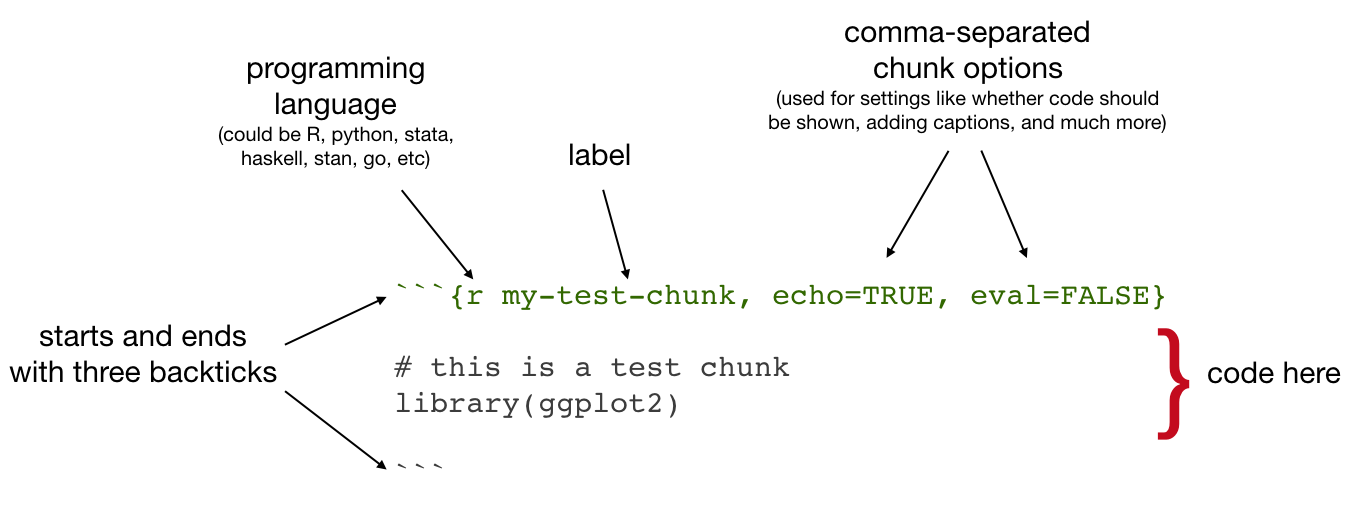
\includegraphics[width=1\linewidth]{figures/chunk-parts} 

}

\caption{Chunk anatomy (https://ulyngs.github.io/rmarkdown-workshop-2019 에서 발췌)}\label{fig:r-code-chunk}
\end{figure}

\normalsize

\hypertarget{code-chunk}{%
\subsection*{자주 활용하는 chunk 옵션}\label{code-chunk}}


\textbf{코드 실행 관련 청크}

\footnotesize

\begin{table}[H]

\caption{\label{tab:chunk-tab-01}코드 실행 관련 청크}
\centering
\fontsize{11}{13}\selectfont
\begin{tabular}[t]{>{\raggedright\arraybackslash}p{3cm}>{\raggedright\arraybackslash}p{3cm}>{\raggedright\arraybackslash}p{8cm}}
\toprule
Chunk 옵션 & Default & 설명\\
\midrule
\rowcolor{gray!6}  eval & TRUE & R 실행(코드 실행 결과)에 대응하는 결과 출력 여부\\
include & TRUE & 출력 문서에 코드 청크의 내용을 포함할지 여부\\
\bottomrule
\end{tabular}
\end{table}

\normalsize

\begin{Shaded}
\begin{Highlighting}[]
\BaseNTok{```\{r ex01-1, eval=TRUE\}}
\BaseNTok{summary(iris)}
\BaseNTok{hist(iris$Sepal.Length)}
\BaseNTok{```}

\BaseNTok{```\{r ex01-2, eval=FALSE\}}
\BaseNTok{summary(iris)}
\BaseNTok{hist(iris$Sepal.Length)}
\BaseNTok{```}
\end{Highlighting}
\end{Shaded}

\footnotesize

\begin{Shaded}
\begin{Highlighting}[]
\CommentTok{#청크 옵션 eval=TRUE}
\KeywordTok{summary}\NormalTok{(iris)}
\end{Highlighting}
\end{Shaded}

\begin{verbatim}
  Sepal.Length    Sepal.Width     Petal.Length    Petal.Width   
 Min.   :4.300   Min.   :2.000   Min.   :1.000   Min.   :0.100  
 1st Qu.:5.100   1st Qu.:2.800   1st Qu.:1.600   1st Qu.:0.300  
 Median :5.800   Median :3.000   Median :4.350   Median :1.300  
 Mean   :5.843   Mean   :3.057   Mean   :3.758   Mean   :1.199  
 3rd Qu.:6.400   3rd Qu.:3.300   3rd Qu.:5.100   3rd Qu.:1.800  
 Max.   :7.900   Max.   :4.400   Max.   :6.900   Max.   :2.500  
       Species  
 setosa    :50  
 versicolor:50  
 virginica :50  
                
                
                
\end{verbatim}

\begin{Shaded}
\begin{Highlighting}[]
\KeywordTok{hist}\NormalTok{(iris}\OperatorTok{$}\NormalTok{Sepal.Length)}
\end{Highlighting}
\end{Shaded}

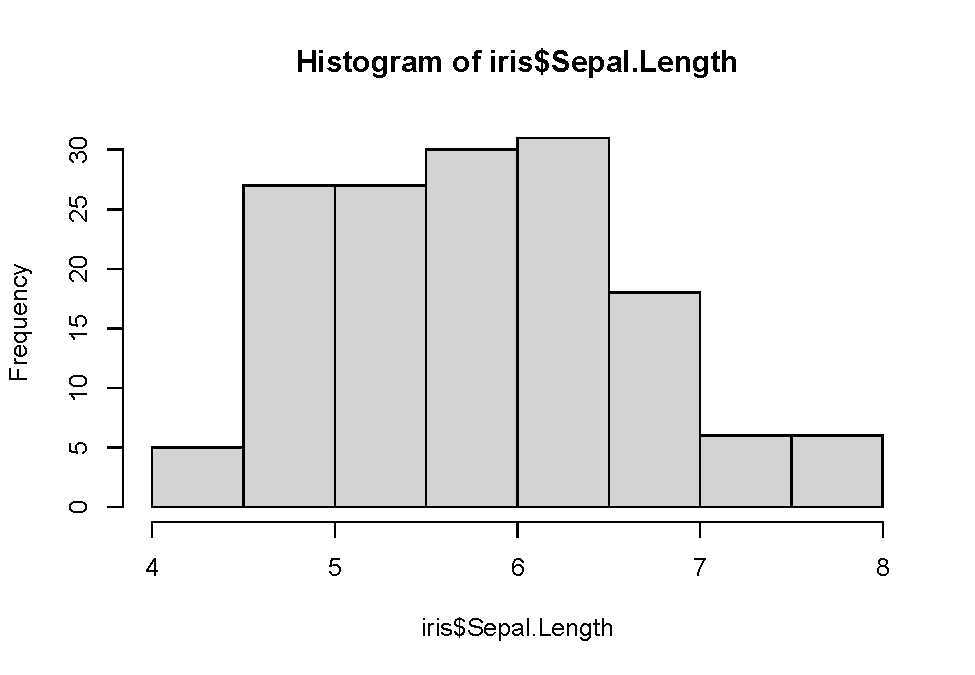
\includegraphics{01-Rmarkdown-1st_files/figure-latex/ex01-1-1.pdf}

\normalsize

\footnotesize

\begin{Shaded}
\begin{Highlighting}[]
\CommentTok{#청크 옵션 eval=FALSE}
\KeywordTok{summary}\NormalTok{(iris)}
\KeywordTok{hist}\NormalTok{(iris}\OperatorTok{$}\NormalTok{Sepal.Length)}
\end{Highlighting}
\end{Shaded}

\normalsize

\textbf{소스 코드 출력(텍스트) 결과 관련 청크}

\footnotesize

\begin{table}[H]

\caption{\label{tab:chunk-tab-02}소스 코드 출력 결과 관련 청크}
\centering
\fontsize{11}{13}\selectfont
\begin{tabular}[t]{>{\raggedright\arraybackslash}p{3cm}>{\raggedright\arraybackslash}p{3cm}>{\raggedright\arraybackslash}p{8cm}}
\toprule
Chunk 옵션 & Default & 설명\\
\midrule
\rowcolor{gray!6}  echo & TRUE & R 실행 결과에 대응하는 코드 출력 여부\\
results & markup & 출력 결과 포맷 지정을 위한 옵션으로 추가적으로 3 가지 옵션 선택 가능: 'hide', 'asis', 'hold', 'markup'\\
\rowcolor{gray!6}  error & TRUE & 코드 또는 스크립트에 구문오류 메세지 출력 여부\\
message & TRUE & 코드로부터 생성된 메세지 출력 여부\\
\rowcolor{gray!6}  warning & TRUE & 경고 메세지 출력 여부\\
\bottomrule
\end{tabular}
\end{table}

\normalsize

\begin{itemize}
\tightlist
\item
  \texttt{echo}: 코드 청크에 작성한 R-script 출력 여부 결정

  \begin{itemize}
  \tightlist
  \item
    \texttt{echo\ =\ FALSE} 이면 소스 코드 출력 없이 그림 결과만 출력
  \end{itemize}
\end{itemize}

\begin{Shaded}
\begin{Highlighting}[]
\BaseNTok{```\{r ex01-2, echo=TRUE\}}
\BaseNTok{require(ggthemes) # ggtheme 패키지 불러오기}
\BaseNTok{require(ggpubr) # ggpubr 패키지 불러오기}
\BaseNTok{iris %>%}
\BaseNTok{   ggplot(aes(x = Sepal.Length, y = Petal.Width, color = Species)) +}
\BaseNTok{   geom_point(size = 5) +}
\BaseNTok{   theme_pubclean() +}
\BaseNTok{   theme(axis.line = element_line(size = 0.8),}
\BaseNTok{         legend.title = element_text(face = "bold", size = 15),}
\BaseNTok{         legend.text = element_text(face = "bold", size = 12))}

\BaseNTok{```}


\BaseNTok{```\{r ex01-3, echo=FALSE\}}
\BaseNTok{require(ggthemes) # ggtheme 패키지 불러오기}
\BaseNTok{require(ggpubr) # ggpubr 패키지 불러오기}
\BaseNTok{iris %>%}
\BaseNTok{   ggplot(aes(x = Sepal.Length, y = Petal.Width, color = Species)) +}
\BaseNTok{   geom_point(size = 5) +}
\BaseNTok{   theme_pubclean() +}
\BaseNTok{   theme(axis.line = element_line(size = 0.8),}
\BaseNTok{         legend.title = element_text(face = "bold", size = 15),}
\BaseNTok{         legend.text = element_text(face = "bold", size = 12))}

\BaseNTok{```}
\end{Highlighting}
\end{Shaded}

\footnotesize

\begin{Shaded}
\begin{Highlighting}[]
\CommentTok{# echo = TRUE}
\KeywordTok{require}\NormalTok{(ggthemes) }\CommentTok{# ggtheme 패키지 불러오기}
\KeywordTok{require}\NormalTok{(ggpubr) }\CommentTok{# ggpubr 패키지 불러오기}
\NormalTok{iris }\OperatorTok
\StringTok{   }\KeywordTok{ggplot}\NormalTok{(}\KeywordTok{aes}\NormalTok{(}\DataTypeTok{x =}\NormalTok{ Sepal.Length, }\DataTypeTok{y =}\NormalTok{ Petal.Width, }\DataTypeTok{color =}\NormalTok{ Species)) }\OperatorTok{+}
\StringTok{   }\KeywordTok{geom_point}\NormalTok{(}\DataTypeTok{size =} \DecValTok{5}\NormalTok{) }\OperatorTok{+}
\StringTok{   }\KeywordTok{theme_pubclean}\NormalTok{() }\OperatorTok{+}
\StringTok{   }\KeywordTok{theme}\NormalTok{(}\DataTypeTok{axis.line =} \KeywordTok{element_line}\NormalTok{(}\DataTypeTok{size =} \FloatTok{0.8}\NormalTok{),}
         \DataTypeTok{legend.title =} \KeywordTok{element_text}\NormalTok{(}\DataTypeTok{face =} \StringTok{"bold"}\NormalTok{, }\DataTypeTok{size =} \DecValTok{15}\NormalTok{),}
         \DataTypeTok{legend.text =} \KeywordTok{element_text}\NormalTok{(}\DataTypeTok{face =} \StringTok{"bold"}\NormalTok{, }\DataTypeTok{size =} \DecValTok{12}\NormalTok{))}
\end{Highlighting}
\end{Shaded}

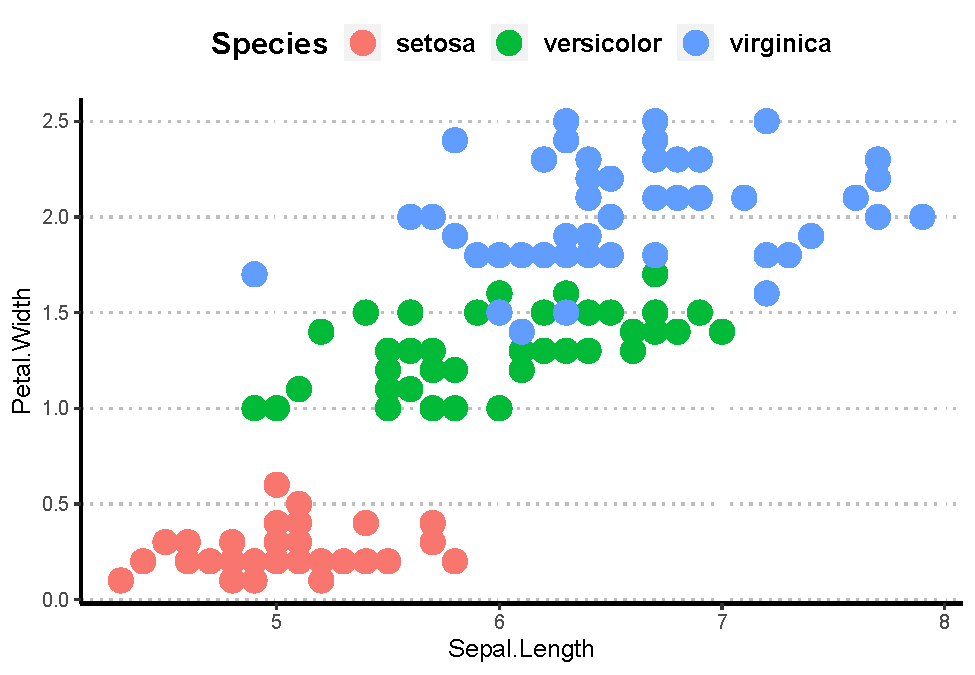
\includegraphics{01-Rmarkdown-1st_files/figure-latex/unnamed-chunk-5-1.pdf}

\normalsize

\begin{itemize}
\tightlist
\item
  \texttt{results}: 코드의 텍스트 출력 결과 포맷 지정

  \begin{itemize}
  \tightlist
  \item
    \texttt{markup} (default): 코드 청크 내 스크립트의 출력 형태에 따라 텍스트 출력 결과를 mark-up
  \item
    \texttt{asis}: 변환하지 않은 원래 R 출력 결과 그대로(as is) 출력
  \item
    \texttt{hide}: R 스크립트로 생성된 텍스트 출력을 보여주지 않음(warning, message 출력 예외)
  \item
    \texttt{hold}: 코드 청크로 생성된 모든 소스 및 출력을 단일 블록으로 축소
  \end{itemize}
\end{itemize}

\footnotesize

\begin{Shaded}
\begin{Highlighting}[]
\CommentTok{# results = 'markup'인 경우 아래 텍스트를 mark-up}
\CommentTok{# (이 경우 아래 텍스트는 ``` ``` 블럭 처리)한 결과를 md 파일로 전송}
\KeywordTok{cat}\NormalTok{(}\StringTok{"I'm raw **Markdown** content.}\CharTok{\textbackslash{}n}\StringTok{"}\NormalTok{)}
\end{Highlighting}
\end{Shaded}

\begin{verbatim}
I'm raw **Markdown** content.
\end{verbatim}

\normalsize

\footnotesize

\begin{figure}

{\centering 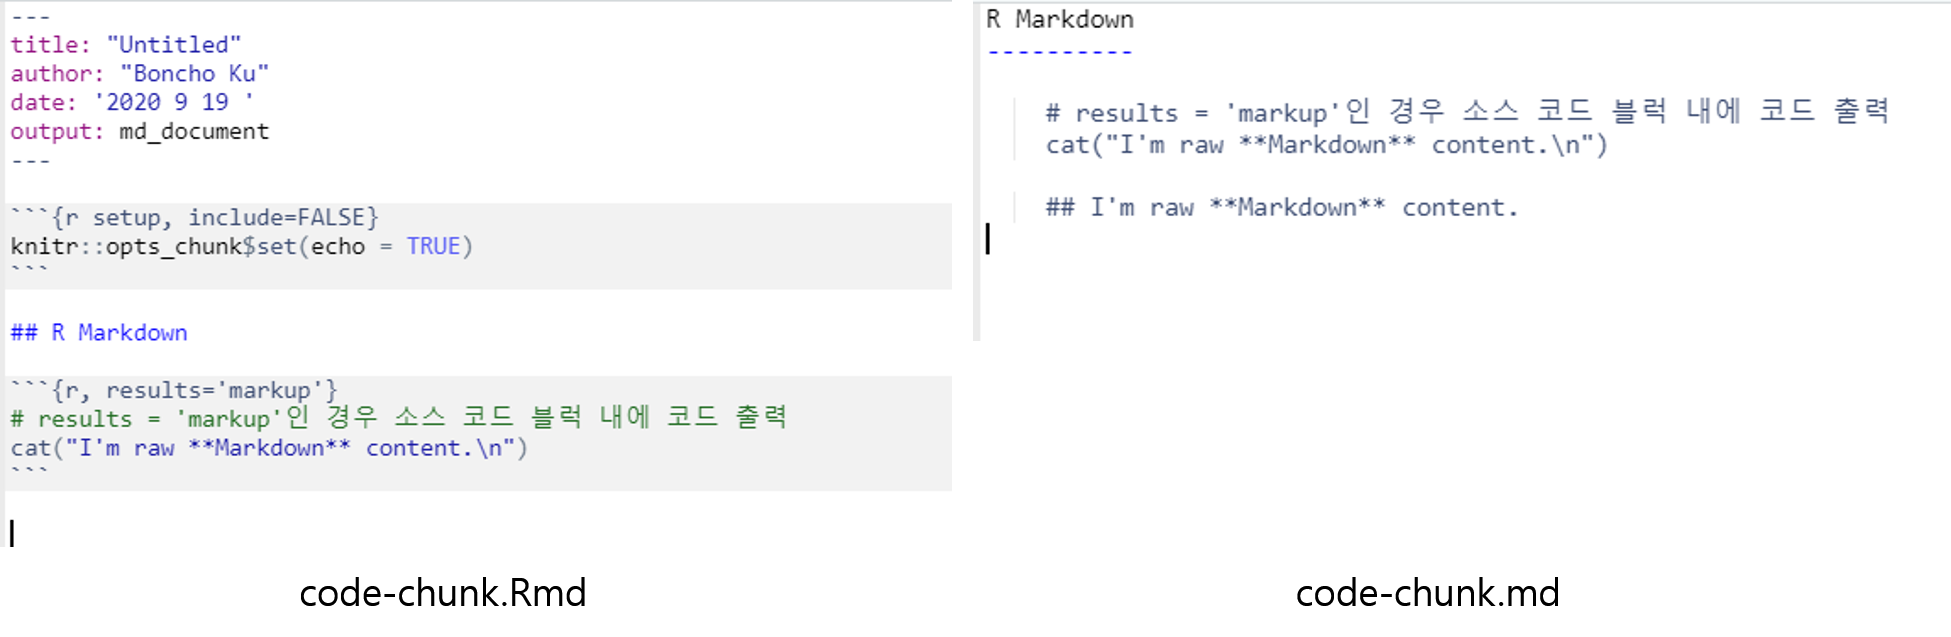
\includegraphics[width=1\linewidth]{figures/code-chunk-markup} 

}

\caption{청크 옵션 results = 'markup'인 경우 rmd vs. md 파일 비교}\label{fig:code-chunk-markup}
\end{figure}

\normalsize

\footnotesize

\begin{Shaded}
\begin{Highlighting}[]
\CommentTok{# results = 'asis' 인 경우 텍스트를 그대로 md 파일에 입력}
\KeywordTok{cat}\NormalTok{(}\StringTok{"I'm raw **Markdown** content.}\CharTok{\textbackslash{}n}\StringTok{"}\NormalTok{)}
\end{Highlighting}
\end{Shaded}

I'm raw \textbf{Markdown} content.

\normalsize

\footnotesize

\begin{figure}

{\centering 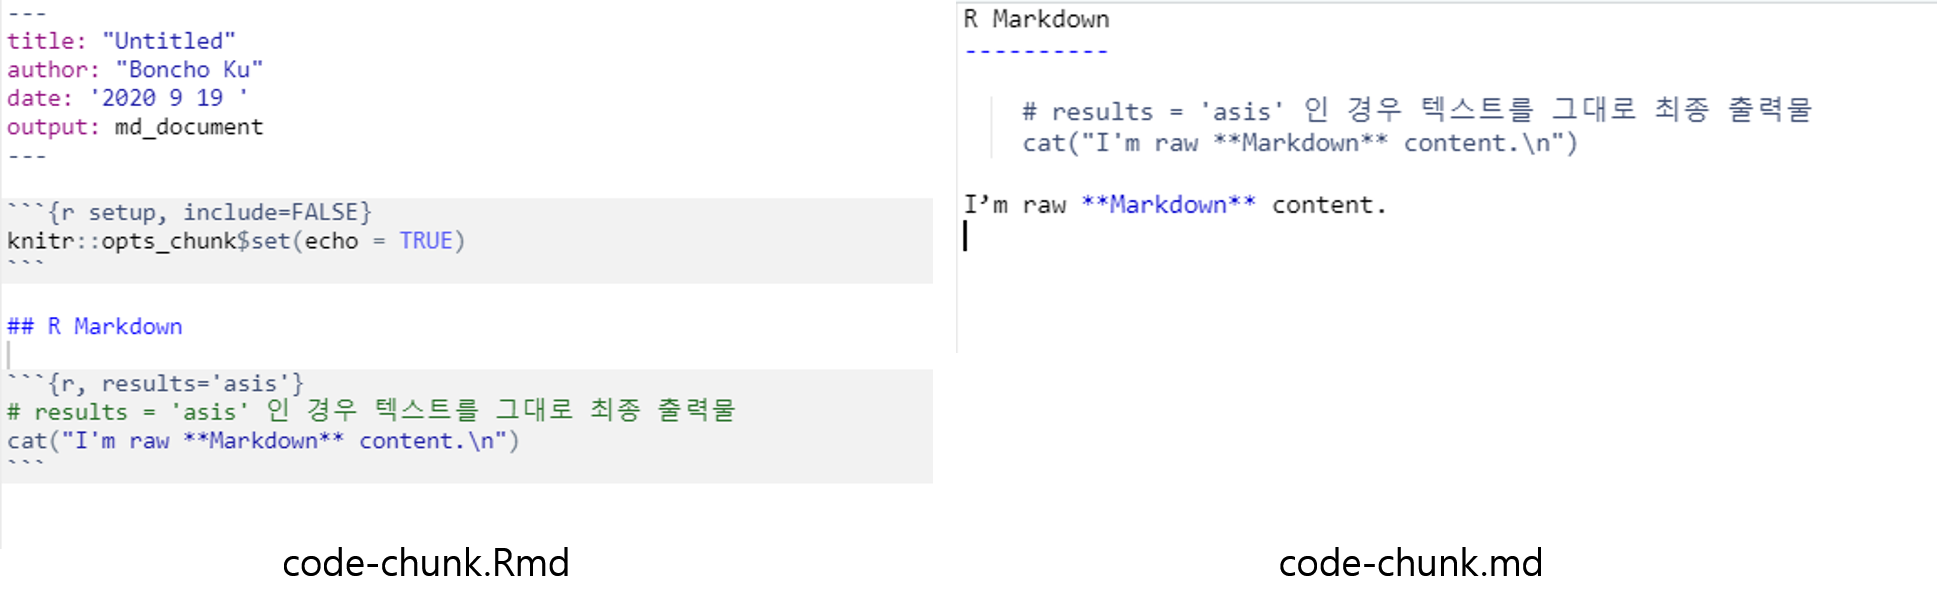
\includegraphics[width=1\linewidth]{figures/code-chunk-asis} 

}

\caption{청크 옵션 results = 'asis'인 경우 rmd vs. md 파일 비교}\label{fig:code-chunk-asis}
\end{figure}

\normalsize

\footnotesize

\begin{Shaded}
\begin{Highlighting}[]
\CommentTok{# results = 'hide'}
\KeywordTok{cat}\NormalTok{(}\StringTok{"I'm raw **Markdown** content.}\CharTok{\textbackslash{}n}\StringTok{"}\NormalTok{)}

\CommentTok{# 텍스트 결과를 출력하지 않음}
\end{Highlighting}
\end{Shaded}

\normalsize

\footnotesize

\begin{Shaded}
\begin{Highlighting}[]
\CommentTok{# results = 'hold'가 아닌 경우 한 라인 별 출력 결과 생성}
\NormalTok{x <-}\StringTok{ }\KeywordTok{rnorm}\NormalTok{(}\DecValTok{10}\NormalTok{)}
\NormalTok{x}
\end{Highlighting}
\end{Shaded}

\begin{verbatim}
 [1]  0.11397949 -1.11975525 -0.39546848 -1.48319594  0.86714230 -0.65739039
 [7] -0.94070684 -0.06004431 -0.84747143  0.11357520
\end{verbatim}

\begin{Shaded}
\begin{Highlighting}[]
\NormalTok{y <-}\StringTok{ }\KeywordTok{rnorm}\NormalTok{(}\DecValTok{10}\NormalTok{, }\DecValTok{1}\NormalTok{, }\DecValTok{2}\NormalTok{)}
\NormalTok{y}
\end{Highlighting}
\end{Shaded}

\begin{verbatim}
 [1]  2.6074654  2.2176548 -1.4640987  1.3247515  1.2189210 -0.5720802
 [7] -0.8809272 -1.9154795 -1.5656312  0.8735466
\end{verbatim}

\begin{Shaded}
\begin{Highlighting}[]
\NormalTok{x }\OperatorTok{+}\StringTok{ }\NormalTok{y}
\end{Highlighting}
\end{Shaded}

\begin{verbatim}
 [1]  2.7214449  1.0978996 -1.8595671 -0.1584444  2.0860633 -1.2294706
 [7] -1.8216340 -1.9755238 -2.4131027  0.9871218
\end{verbatim}

\normalsize

\footnotesize

\begin{Shaded}
\begin{Highlighting}[]
\CommentTok{# results = 'hold'인 경우 코드 부분과 출력 부분이 따로 블록 처리}
\NormalTok{x <-}\StringTok{ }\KeywordTok{rnorm}\NormalTok{(}\DecValTok{10}\NormalTok{)}
\NormalTok{x}
\NormalTok{y <-}\StringTok{ }\KeywordTok{rnorm}\NormalTok{(}\DecValTok{10}\NormalTok{, }\DecValTok{1}\NormalTok{, }\DecValTok{2}\NormalTok{)}
\NormalTok{y}
\NormalTok{x }\OperatorTok{+}\StringTok{ }\NormalTok{y}
\end{Highlighting}
\end{Shaded}

\begin{verbatim}
 [1] -1.0223661  0.2992861 -1.1081556 -0.0126041 -1.1982391 -1.5091321
 [7] -0.8100077 -0.9633556  0.6873936  0.1792799
 [1] -3.37265758  0.97343197 -0.02659187  1.06986991  5.90701592  0.33479442
 [7]  0.74497495 -1.38770572  2.16830646  2.78405177
 [1] -4.39502367  1.27271807 -1.13474743  1.05726582  4.70877684 -1.17433764
 [7] -0.06503275 -2.35106137  2.85570008  2.96333162
\end{verbatim}

\normalsize

\begin{itemize}
\tightlist
\item
  \texttt{error}: 코드 청크 내 스크립트에 오류에 대한 보존 여부(\texttt{stop()})

  \begin{itemize}
  \tightlist
  \item
    기본적으로 Rmarkdown 컴파일 시 \texttt{error}에 대한 옵션이 \texttt{FALSE}이기 때문에 스크립트(코드)에 오류가 포함되면 컴파일이 정지됨.
  \item
    \texttt{error\ =\ TRUE} 이면 오류 메세지를 포함한 텍스트 결과를 출력
  \end{itemize}
\end{itemize}

\footnotesize

\begin{Shaded}
\begin{Highlighting}[]
\NormalTok{3x <-}\StringTok{ }\DecValTok{3}
\NormalTok{x <-}\StringTok{ }\DecValTok{25} \CommentTok{# 위 행이 구문 오류를 포함하고 있기 때문에}
        \CommentTok{# 오류 이후의 코드는 실행되지 않음}
\NormalTok{x}
\end{Highlighting}
\end{Shaded}

\begin{verbatim}
Error: <text>:1:2: 예상하지 못한 기호(symbol)입니다.
1: 3x
     ^
\end{verbatim}

\normalsize

\begin{itemize}
\tightlist
\item
  \texttt{message}/\texttt{warning}: 텍스트 출력물 중 경고(warning, \texttt{warning()} 함수의 출력 결과) 메세지 출력 여부 결정
\end{itemize}

\footnotesize

\begin{Shaded}
\begin{Highlighting}[]
\CommentTok{# message = TRUE 인 경우 함수 message 출력}
\NormalTok{testit <-}\StringTok{ }\ControlFlowTok{function}\NormalTok{() \{}
  \KeywordTok{message}\NormalTok{(}\StringTok{"testing package startup messages"}\NormalTok{)}
  \KeywordTok{packageStartupMessage}\NormalTok{(}\StringTok{"initializing ..."}\NormalTok{, }\DataTypeTok{appendLF =} \OtherTok{FALSE}\NormalTok{)}
  \KeywordTok{Sys.sleep}\NormalTok{(}\DecValTok{1}\NormalTok{)}
  \KeywordTok{packageStartupMessage}\NormalTok{(}\StringTok{" done"}\NormalTok{)}
\NormalTok{\} }\CommentTok{# help(message) 예시 중 발췌}

\KeywordTok{testit}\NormalTok{()}
\end{Highlighting}
\end{Shaded}

\begin{verbatim}
testing package startup messages
\end{verbatim}

\begin{verbatim}
initializing ... done
\end{verbatim}

\normalsize

\footnotesize

\begin{Shaded}
\begin{Highlighting}[]
\CommentTok{# message=FALSE -> 메세지 출력하지 않음}
\KeywordTok{testit}\NormalTok{()}
\end{Highlighting}
\end{Shaded}

\normalsize

\footnotesize

\begin{Shaded}
\begin{Highlighting}[]
\CommentTok{# 경고 메세지 출력}
\NormalTok{x <-}\StringTok{ }\KeywordTok{c}\NormalTok{(}\DecValTok{1}\NormalTok{, }\DecValTok{2}\NormalTok{, }\StringTok{"new"}\NormalTok{, }\DecValTok{4}\OperatorTok{:}\DecValTok{10}\NormalTok{)}
\NormalTok{x <-}\StringTok{ }\KeywordTok{as.numeric}\NormalTok{(x)}
\end{Highlighting}
\end{Shaded}

\begin{verbatim}
Warning: 강제형변환에 의해 생성된 NA 입니다
\end{verbatim}

\normalsize

\textbf{코드 서식 관련 청크 옵션}

\footnotesize

\begin{table}[H]

\caption{\label{tab:chunk-tab-03}코드 서식 관련 청크}
\centering
\fontsize{11}{13}\selectfont
\begin{tabular}[t]{>{\raggedright\arraybackslash}p{3cm}>{\raggedright\arraybackslash}p{3cm}>{\raggedright\arraybackslash}p{8cm}}
\toprule
Chunk 옵션 & Default & 설명\\
\midrule
\rowcolor{gray!6}  comment & TRUE & 소스 코드 실행 출력의 각 줄 앞에 붙는 표시문자 출력 여부: 기본 값은 '\#\#' 임\\
highlight & TRUE & 구문 강조 여부\\
\rowcolor{gray!6}  prompt & FALSE & R 프롬프트 출력 여부\\
tidy & FALSE & R 소스 코드 출력 정리 여부\\
\bottomrule
\end{tabular}
\end{table}

\normalsize

\begin{itemize}
\tightlist
\item
  \texttt{comment}: 텍스트 출력물에 주석 표시(default)를 함으로써 소스 코드와 출력 결과를 동시 선택과 복사를 가능(\#\#는 주석 표시이기 때문에 실행되지 않음)

  \begin{itemize}
  \tightlist
  \item
    주석 표시를 제거하고 싶다면 \texttt{comment\ =\ NA} 또는 \texttt{comment\ =\ \textquotesingle{}\textquotesingle{}}
  \end{itemize}
\end{itemize}

\footnotesize

\begin{Shaded}
\begin{Highlighting}[]
\CommentTok{# 디폴트 comment 사용}
\KeywordTok{summary}\NormalTok{(iris)}
\end{Highlighting}
\end{Shaded}

\begin{verbatim}
##   Sepal.Length    Sepal.Width     Petal.Length    Petal.Width   
##  Min.   :4.300   Min.   :2.000   Min.   :1.000   Min.   :0.100  
##  1st Qu.:5.100   1st Qu.:2.800   1st Qu.:1.600   1st Qu.:0.300  
##  Median :5.800   Median :3.000   Median :4.350   Median :1.300  
##  Mean   :5.843   Mean   :3.057   Mean   :3.758   Mean   :1.199  
##  3rd Qu.:6.400   3rd Qu.:3.300   3rd Qu.:5.100   3rd Qu.:1.800  
##  Max.   :7.900   Max.   :4.400   Max.   :6.900   Max.   :2.500  
##        Species  
##  setosa    :50  
##  versicolor:50  
##  virginica :50  
##                 
##                 
## 
\end{verbatim}

\normalsize

\begin{itemize}
\tightlist
\item
  \texttt{highlight}: 구문 강조 표시 여부

  \begin{itemize}
  \tightlist
  \item
    \texttt{highlight=FALSE} 일 때 소스 코드 출력 결과
  \end{itemize}
\end{itemize}

\footnotesize

\begin{verbatim}
# highlight=FALSE

iris %>%
   ggplot(aes(x = Sepal.Length, y = Petal.Width, color = Species)) +
   geom_point(size = 5) +
   theme_pubclean() +
   theme(axis.line = element_line(size = 0.8),
         legend.title = element_text(face = "bold", size = 15),
         legend.text = element_text(face = "bold", size = 12))
\end{verbatim}

\normalsize

\begin{itemize}
\tightlist
\item
  \texttt{prompt}: R 콘솔 상 프롬프트 \texttt{\textgreater{}}, \texttt{+} 출력 여부
\end{itemize}

\footnotesize

\begin{Shaded}
\begin{Highlighting}[]
\OperatorTok{>}\StringTok{ }\CommentTok{# prompt = TRUE 인 경우 코드 출력 결과}
\ErrorTok{>}\StringTok{ }\KeywordTok{require}\NormalTok{(ggthemes) }\CommentTok{# ggtheme 패키지 불러오기}
\OperatorTok{>}\StringTok{ }\KeywordTok{require}\NormalTok{(ggpubr) }\CommentTok{# ggpubr 패키지 불러오기}
\OperatorTok{>}\StringTok{ }\NormalTok{iris }\OperatorTok
\OperatorTok{+}\StringTok{    }\KeywordTok{ggplot}\NormalTok{(}\KeywordTok{aes}\NormalTok{(}\DataTypeTok{x =}\NormalTok{ Sepal.Length, }\DataTypeTok{y =}\NormalTok{ Petal.Width, }\DataTypeTok{color =}\NormalTok{ Species)) }\OperatorTok{+}
\OperatorTok{+}\StringTok{    }\KeywordTok{geom_point}\NormalTok{(}\DataTypeTok{size =} \DecValTok{5}\NormalTok{) }\OperatorTok{+}
\OperatorTok{+}\StringTok{    }\KeywordTok{theme_pubclean}\NormalTok{() }\OperatorTok{+}
\OperatorTok{+}\StringTok{    }\KeywordTok{theme}\NormalTok{(}\DataTypeTok{axis.line =} \KeywordTok{element_line}\NormalTok{(}\DataTypeTok{size =} \FloatTok{0.8}\NormalTok{),}
\OperatorTok{+}\StringTok{          }\DataTypeTok{legend.title =} \KeywordTok{element_text}\NormalTok{(}\DataTypeTok{face =} \StringTok{"bold"}\NormalTok{, }\DataTypeTok{size =} \DecValTok{15}\NormalTok{),}
\OperatorTok{+}\StringTok{          }\DataTypeTok{legend.text =} \KeywordTok{element_text}\NormalTok{(}\DataTypeTok{face =} \StringTok{"bold"}\NormalTok{, }\DataTypeTok{size =} \DecValTok{12}\NormalTok{))}
\end{Highlighting}
\end{Shaded}

\normalsize

\begin{itemize}
\tightlist
\item
  \texttt{tidy}: 코드를 사용자가 지정(혹은 \texttt{formatR::tidy\_sorce()} 함수에 초기값으로 지정된 코드 정리 값)한 줄 당 문자 길이 등을 반영해 코드를 정리

  \begin{itemize}
  \tightlist
  \item
    \texttt{tidy=TRUE} 인 경우 자동으로 줄 바꿈
  \end{itemize}
\end{itemize}

\footnotesize

\begin{Shaded}
\begin{Highlighting}[]
\OperatorTok{>}\StringTok{ }\CommentTok{# tidy = FALSE 인 경우 코드 출력 결과}
\ErrorTok{>}\StringTok{ }\KeywordTok{require}\NormalTok{(ggthemes) }\CommentTok{# ggtheme 패키지 불러오기}
\OperatorTok{>}\StringTok{ }\KeywordTok{require}\NormalTok{(ggpubr) }\CommentTok{# ggpubr 패키지 불러오기}
\OperatorTok{>}\StringTok{ }\NormalTok{iris }\OperatorTok\StringTok{ }\KeywordTok{ggplot}\NormalTok{(}\KeywordTok{aes}\NormalTok{(}\DataTypeTok{x =}\NormalTok{ Sepal.Length, }\DataTypeTok{y =}\NormalTok{ Petal.Width, }\DataTypeTok{color =}\NormalTok{ Species)) }\OperatorTok{+}\StringTok{ }\KeywordTok{geom_point}\NormalTok{(}\DataTypeTok{size =} \DecValTok{5}\NormalTok{) }\OperatorTok{+}\StringTok{ }\KeywordTok{theme_pubclean}\NormalTok{() }\OperatorTok{+}\StringTok{ }\KeywordTok{theme}\NormalTok{(}\DataTypeTok{axis.line =} \KeywordTok{element_line}\NormalTok{(}\DataTypeTok{size =} \FloatTok{0.8}\NormalTok{), }\DataTypeTok{legend.title =} \KeywordTok{element_text}\NormalTok{(}\DataTypeTok{face =} \StringTok{"bold"}\NormalTok{, }\DataTypeTok{size =} \DecValTok{15}\NormalTok{), }\DataTypeTok{legend.text =} \KeywordTok{element_text}\NormalTok{(}\DataTypeTok{face =} \StringTok{"bold"}\NormalTok{, }\DataTypeTok{size =} \DecValTok{12}\NormalTok{))}
\end{Highlighting}
\end{Shaded}

\normalsize

\footnotesize

\begin{Shaded}
\begin{Highlighting}[]
\OperatorTok{>}\StringTok{ }\CommentTok{# tidy = TRUE 인 경우 코드 출력 결과}
\ErrorTok{>}\StringTok{ }\KeywordTok{require}\NormalTok{(ggthemes)  }\CommentTok{# ggtheme 패키지 불러오기}
\OperatorTok{>}\StringTok{ }\KeywordTok{require}\NormalTok{(ggpubr)  }\CommentTok{# ggpubr 패키지 불러오기}
\OperatorTok{>}\StringTok{ }\NormalTok{iris }\OperatorTok\StringTok{ }\KeywordTok{ggplot}\NormalTok{(}\KeywordTok{aes}\NormalTok{(}\DataTypeTok{x =}\NormalTok{ Sepal.Length, }\DataTypeTok{y =}\NormalTok{ Petal.Width, }\DataTypeTok{color =}\NormalTok{ Species)) }\OperatorTok{+}\StringTok{ }\KeywordTok{geom_point}\NormalTok{(}\DataTypeTok{size =} \DecValTok{5}\NormalTok{) }\OperatorTok{+}\StringTok{ }
\OperatorTok{+}\StringTok{     }\KeywordTok{theme_pubclean}\NormalTok{() }\OperatorTok{+}\StringTok{ }\KeywordTok{theme}\NormalTok{(}\DataTypeTok{axis.line =} \KeywordTok{element_line}\NormalTok{(}\DataTypeTok{size =} \FloatTok{0.8}\NormalTok{), }\DataTypeTok{legend.title =} \KeywordTok{element_text}\NormalTok{(}\DataTypeTok{face =} \StringTok{"bold"}\NormalTok{, }
\OperatorTok{+}\StringTok{     }\DataTypeTok{size =} \DecValTok{15}\NormalTok{), }\DataTypeTok{legend.text =} \KeywordTok{element_text}\NormalTok{(}\DataTypeTok{face =} \StringTok{"bold"}\NormalTok{, }\DataTypeTok{size =} \DecValTok{12}\NormalTok{))}
\end{Highlighting}
\end{Shaded}

\normalsize

\textbf{그림(plot) 출력 관련 청크 옵션}

\footnotesize

\begin{table}[H]

\caption{\label{tab:chunk-tab-04}Plot 출력 관련 청크}
\centering
\fontsize{11}{13}\selectfont
\begin{tabular}[t]{>{\raggedright\arraybackslash}p{5cm}>{\raggedright\arraybackslash}p{5cm}>{\raggedright\arraybackslash}p{8cm}}
\toprule
Chunk 옵션 & Default & 설명\\
\midrule
\rowcolor{gray!6}  fig.align & default & 최종 문서에 plot 정렬 방식 결정(center/left/right)\\
fig.height/fig.width & 7 & 그림 크기(단위: 인치)\\
\rowcolor{gray!6}  fig.cap & NULL & 그림 캡션(문자열 입력)\\
dpi & 72 & dot per inche: 출력 그림 해상도\\
\bottomrule
\end{tabular}
\end{table}

\normalsize

\hypertarget{typical-chunk}{%
\subsection*{알아두면 좋은 청크 형태}\label{typical-chunk}}


\textbf{Setup 청크}

\begin{itemize}
\tightlist
\item
  일반적으로 Rmarkdown 문서는 YAML 해더 뒤에 전역적 청크 옵션 지정과 R 패키지를 불러오는 것으로 시작
\item
  청크 옵션은 \texttt{knitr::opts\_chunk\$set(청크\ 옵션\ 지정)} 형태로 지정 가능
\item
  다음은 RStudio 에서 Rmd 문서 생성 시 맨 처음 나오는 코드 청크 예시임
\end{itemize}

\begin{Shaded}
\begin{Highlighting}[]
\BaseNTok{```\{r ex01-2, include=FALSE\}}
\BaseNTok{knitr::opts_chunk$set(echo = TRUE)}
\BaseNTok{```}
\end{Highlighting}
\end{Shaded}

\begin{itemize}
\tightlist
\item
  일반적 활용 예시
\end{itemize}

\begin{Shaded}
\begin{Highlighting}[]
\BaseNTok{```\{r option-init, include=FALSE\}}
\BaseNTok{knitr::opts_chunk$set(root.dir = '../..', # 프로젝트 폴더 지정}
\BaseNTok{                      eval = TRUE,}
\BaseNTok{                      echo = FALSE,}
\BaseNTok{                      cache = FALSE,}
\BaseNTok{                      include = TRUE,}
\BaseNTok{                      tidy = TRUE,}
\BaseNTok{                      tidy.opts = list(blank=FALSE, width.cutoff=120), # 소스 출력길이 지정}
\BaseNTok{                      message = FALSE,}
\BaseNTok{                      warning = FALSE,}
\BaseNTok{                      engine = "R", # Chunks will always have R code, unless noted}
\BaseNTok{                      error = TRUE,}
\BaseNTok{                      fig.path="Figures/",  # Set the figure options}
\BaseNTok{                      fig.align = "center",}
\BaseNTok{                      fig.width = 7,}
\BaseNTok{                      fig.height = 7,}
\BaseNTok{                      fig.keep='all', fig.retina=2)}
\BaseNTok{```}
\end{Highlighting}
\end{Shaded}

\textbf{이미지 불러오기}

\begin{Shaded}
\begin{Highlighting}[]
\BaseNTok{```\{r, fig.cap = "Taj Mahal"\}}
\BaseNTok{knitr::include_graphics("figures/taj.JPG", dpi = NA)}
\BaseNTok{```}
\end{Highlighting}
\end{Shaded}

\footnotesize

\begin{figure}
\centering
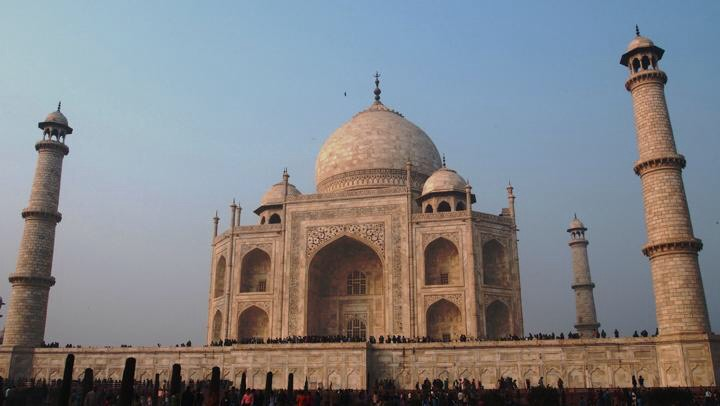
\includegraphics{figures/taj.JPG}
\caption{\label{fig:unnamed-chunk-20}Taj Mahal}
\end{figure}

\normalsize

\begin{Shaded}
\begin{Highlighting}[]
\BaseNTok{```\{r, fig.cap = "Taj Mahal"\}}
\BaseNTok{cars %>%}
\BaseNTok{   ggplot(aes(x = speed, y = dist)) +}
\BaseNTok{   geom_point(size = 5) +}
\BaseNTok{   theme_tufte(base_size = 15) # ggtheme::theme_tufte()}
\BaseNTok{```}
\end{Highlighting}
\end{Shaded}

\textbf{R 생성 도표 포함}

\footnotesize

\begin{figure}
\centering
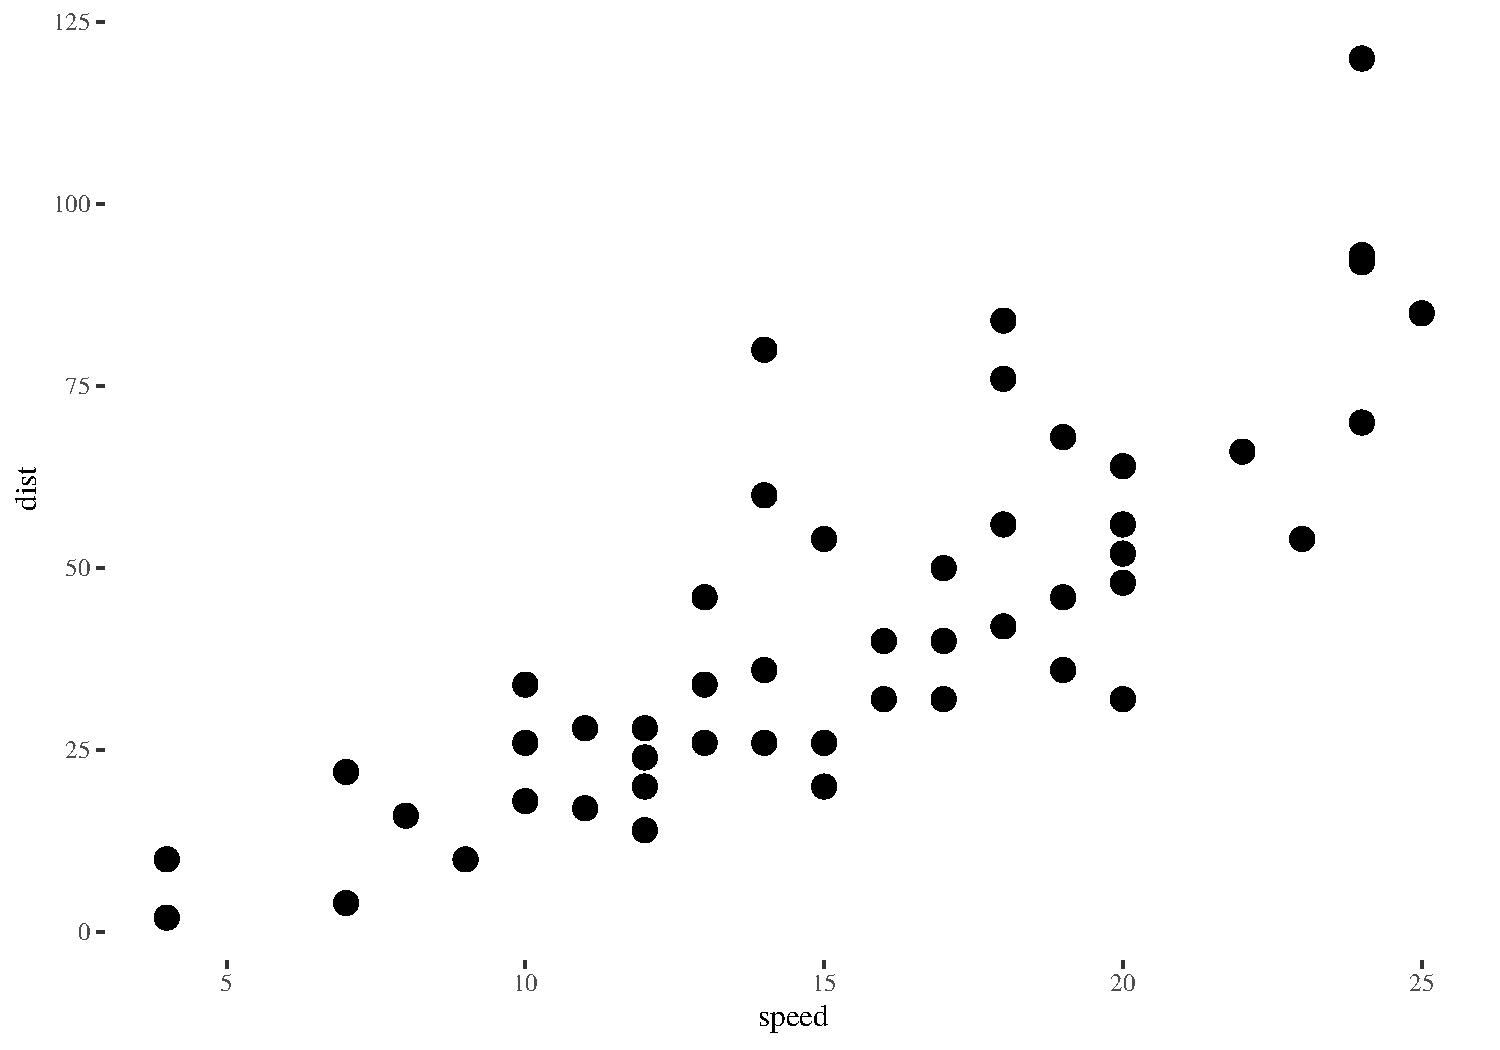
\includegraphics{01-Rmarkdown-1st_files/figure-latex/plot-example-1.pdf}
\caption{\label{fig:plot-example}Scatterplot of the car dataset}
\end{figure}

\normalsize

\textbf{테이블 삽입}

\begin{itemize}
\tightlist
\item
  가장 간단한 테이블은 \texttt{knitr::kable()} 함수를 통해 생성 가능
\item
  \texttt{kable()} 함수는 가장 단순한 형태의 표만 생성하기 때문에 복잡한 표를 만들기에는 한계가 존재함
\item
  이를 보완하기 위해 다음과 같은 패키지 활용

  \begin{itemize}
  \tightlist
  \item
    \texttt{kableExtra}: HTML 또는 LaTeX 용 표 생성

    \begin{itemize}
    \tightlist
    \item
      \url{https://cran.r-project.org/web/packages/kableExtra/vignettes/awesome_table_in_html.html}
    \item
      \url{https://cran.r-project.org/web/packages/kableExtra/vignettes/awesome_table_in_pdf.pdf}
    \end{itemize}
  \item
    \texttt{flextable} + \texttt{officer}: HTML, 워드 문서 표 작성

    \begin{itemize}
    \tightlist
    \item
      \url{https://davidgohel.github.io/flextable/}
    \end{itemize}
  \end{itemize}
\end{itemize}

\begin{Shaded}
\begin{Highlighting}[]
\BaseNTok{```\{r\}}
\BaseNTok{knitr::kable(head(iris))}
\BaseNTok{```}
\end{Highlighting}
\end{Shaded}

\footnotesize

\begin{tabular}{r|r|r|r|l}
\hline
Sepal.Length & Sepal.Width & Petal.Length & Petal.Width & Species\\
\hline
5.1 & 3.5 & 1.4 & 0.2 & setosa\\
\hline
4.9 & 3.0 & 1.4 & 0.2 & setosa\\
\hline
4.7 & 3.2 & 1.3 & 0.2 & setosa\\
\hline
4.6 & 3.1 & 1.5 & 0.2 & setosa\\
\hline
5.0 & 3.6 & 1.4 & 0.2 & setosa\\
\hline
5.4 & 3.9 & 1.7 & 0.4 & setosa\\
\hline
\end{tabular}

\normalsize

\hypertarget{inline-code}{%
\section{인라인(inline) R 코드}\label{inline-code}}

\begin{itemize}
\tightlist
\item
  문서의 모든 숫자를 인라인 R 코드를 통해 재현가능하게 생성 가능
\item
  인라인 R 코드는 \texttt{\textasciigrave{}r} 과 \texttt{\textasciigrave{}} 사이에 변수 계산 스크립트를 입력해 작성 가능
\item
  예를 들어 {`}r 10 + 4` 는 14 출력
\item
  활용 예시
\end{itemize}

\footnotesize

\begin{Shaded}
\begin{Highlighting}[]
\KeywordTok{head}\NormalTok{(mtcars, }\DecValTok{5}\NormalTok{)}
\end{Highlighting}
\end{Shaded}

\begin{verbatim}
                   mpg cyl disp  hp drat    wt  qsec vs am gear carb
Mazda RX4         21.0   6  160 110 3.90 2.620 16.46  0  1    4    4
Mazda RX4 Wag     21.0   6  160 110 3.90 2.875 17.02  0  1    4    4
Datsun 710        22.8   4  108  93 3.85 2.320 18.61  1  1    4    1
Hornet 4 Drive    21.4   6  258 110 3.08 3.215 19.44  1  0    3    1
Hornet Sportabout 18.7   8  360 175 3.15 3.440 17.02  0  0    3    2
\end{verbatim}

\begin{Shaded}
\begin{Highlighting}[]
\NormalTok{N <-}\StringTok{ }\KeywordTok{nrow}\NormalTok{(mtcars)}
\end{Highlighting}
\end{Shaded}

\normalsize

\texttt{mtcars} 데이터셋에 포함된 자동차는 {`}r N ` 개다.

\(\rightarrow\)

\texttt{mtcars} 데이터셋에 포함된 자동차는 32 개다.

\hypertarget{yaml}{%
\section{YAML}\label{yaml}}

\begin{itemize}
\tightlist
\item
  R Markdown 문서의 가장 처음에 정의하는 metadata
\item
  \texttt{.Rmd} 파일을 \texttt{.md} 파일로 변환 후 최종 출력문서 생성 시 필요한 pandoc의 옵션을 설정하는 것과 같은 의미임
\item
  일반적으로 문서 형태 및 생성을 위해 사용하는 R package (예: bookdown, officedown, rticles 등)에 따라 YAML 구성요소가 달라짐
\end{itemize}

\hypertarget{basic-syntax}{%
\subsection*{기본 문법}\label{basic-syntax}}


\begin{itemize}
\tightlist
\item
  /\#: 주석 처리
\item
  YAML 문서의 시작과 끝은 \texttt{-\/-\/-} 로 정의함
\item
  기본적으로 콜론(\texttt{:})으로 구분된 태그(키): 값 쌍으로 구성됨 \(\rightarrow\) \texttt{key:\ value}

  \begin{itemize}
  \tightlist
  \item
    여기서 콜론 바로 다음에는 반드시 공백문자가 있어야 함
  \end{itemize}
\item
  한 \texttt{key}의 하위 키는 리스트 형태로 표현하고, 하위 키는 두 개 이상의 스페이스로 공백을 주어 표현
\end{itemize}

\begin{Shaded}
\begin{Highlighting}[]
\PreprocessorTok{---}
\FunctionTok{key }\KeywordTok{:}\AttributeTok{ value}
\AttributeTok{   }\FunctionTok{subkey1}\KeywordTok{:}\AttributeTok{ value1}
\AttributeTok{   }\FunctionTok{subkey2}\KeywordTok{:}\AttributeTok{ value2}
\AttributeTok{      }\FunctionTok{subsubkey1}\KeywordTok{:}\AttributeTok{ value3}
\PreprocessorTok{---}
\end{Highlighting}
\end{Shaded}

\hypertarget{rmarkdown-yaml-structure}{%
\subsection*{R Markdown 기본 YAML 구조}\label{rmarkdown-yaml-structure}}


\begin{verbatim}
---
title: "문서 제목" # 일반적으로 따옴표 사용
subtitle: "문서 부제목"
author: "문서 작성자"
date: "문서 작성일자" 
output: 
   - "html_document"
   - "word_document"
   - "pdf_document"
   - "md_document"
   - "isoslides_presentation"
   - "slidy_presentation"
   - "beamer_presentation"
bibliography: 참고문헌.bib # bibtex 서식 활용
.
.
.
---
\end{verbatim}

\begin{itemize}
\tightlist
\item
  \url{https://bookdown.org/yihui/rmarkdown/documents.html} 에 자세한 예시 참고
\end{itemize}

\hypertarget{rmarkdown-citation}{%
\section{참고문헌 인용}\label{rmarkdown-citation}}

\begin{itemize}
\tightlist
\item
  참고문헌 정보가 BibTeX 포맷으로 저장된 \texttt{.bib} 파일을 YAML에 선언 후 인용 가능
\end{itemize}

\footnotesize

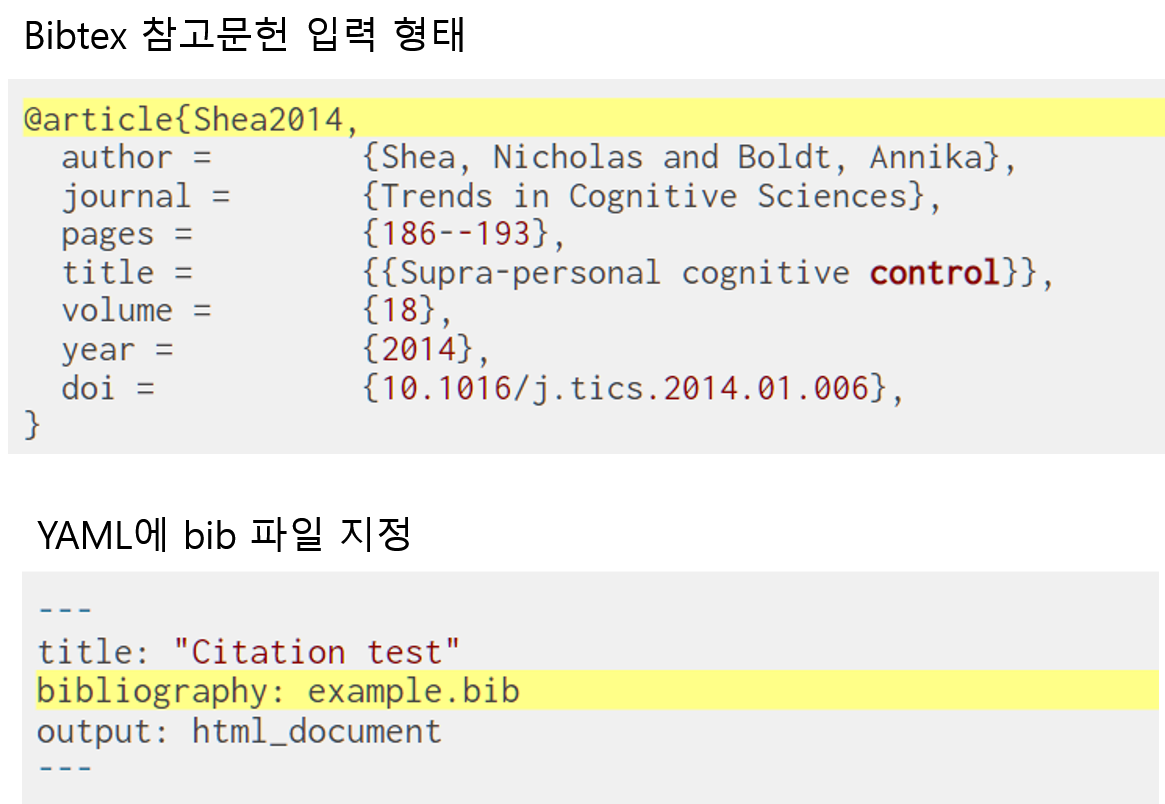
\includegraphics{figures/bibtex-yaml.PNG}

\normalsize

\begin{itemize}
\tightlist
\item
  참고문헌 표현: \texttt{{[}@citation-identifier{]}} 또는 \texttt{@citation-identifier}
\end{itemize}

\footnotesize

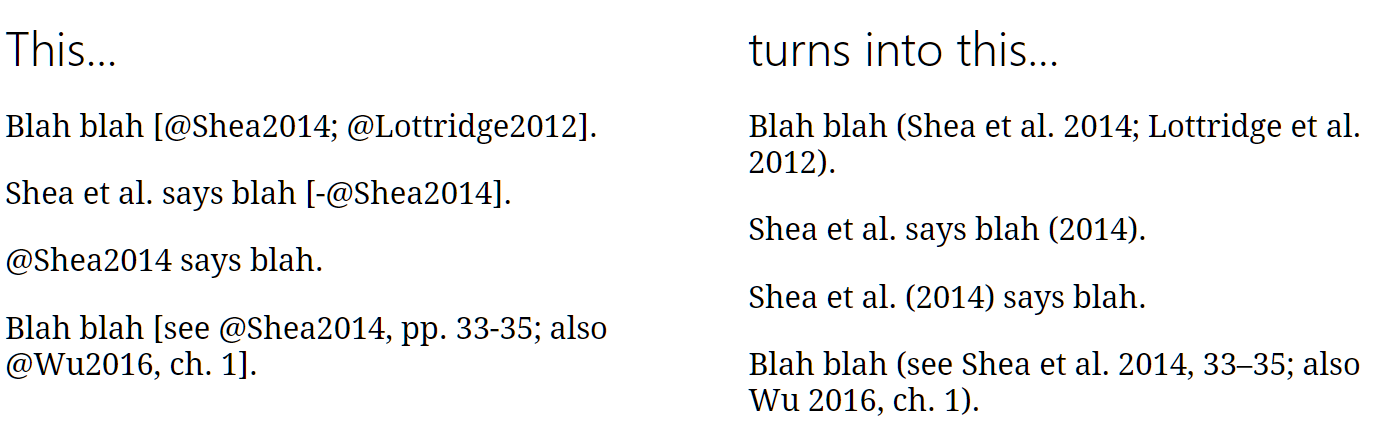
\includegraphics{figures/citationPNG.PNG}

\normalsize

\begin{itemize}
\tightlist
\item
  BibTeX 포맷은 Google Scholar 에서 쉽게 획득 가능
\item
  Citation 스타일은 YAML 헤더에 \texttt{cl:\ style.csl}로 변경 가능하며 \href{https://www.zotero.org}{Zotero} 에서 \texttt{.csl} 파일 다운로드 가능
\end{itemize}

  \bibliography{book.bib,packages.bib}

\printindex

\end{document}
